\chapter{Simplified re-interpretation procedure}\label{app:simplified_reinterp}
This Appendix introduces a simplified approach to \textit{re-interpreting} cross section measurements which is applied to the CMS Higgs boson combination using the HEL parameterisation. This method has been used to investigate particular properties of the HEL interpretation, such as the most important operators for the combination input analyses, and to gain an estimate of their respective sensitivity. A $\chi^2$ function is constructed using measurements from different input analyses,

\begin{equation}
    \chi^2(\vec{c}) = \sum_a (\mathbf{X}_a-\pmb{\mu})^T \mathbf{V}_a^{-1} (\mathbf{X}_a-\pmb{\mu}),
\end{equation}

\noindent
with the following inputs:

\begin{itemize}
    \item $a$: index to label the input analysis.
    \item $\mathbf{X}_a$: a vector of cross section times branching fraction measurements from analysis, $a$. The elements of the vector are the best-fit values of $[\sigma^i\cdot\mathcal{B}^f]_{\rm{obs}}$, relative to the SM prediction: $x^{i,f}_a=[\sigma^i\cdot\mathcal{B}^f]_{\rm{obs}}/[\sigma^i\cdot\mathcal{B}^f]_{\rm{SM}}$. For example, to use the \Hgg minimal merging results shown in Chapter \ref{chap:hgg_results}, $\mathbf{X}_a$ would be a vector of the best-fit values shown in the final column of Table~\ref{tab:stage1p2_minimal_results}.
    \item $\pmb{\mu}$: a vector of EFT scaling functions, $\mu^{i,f}(\vec{c})$, where the elements match the corresponding measurement in the $\mathbf{X}_a$ vector: $x^{i,f}_a$. In this manner, the element-wise subtraction is minimised for the HEL parameter point in which $\mu^{i,f}(\vec{c})=[\sigma^i\cdot\mathcal{B}^f]_{\rm{obs}}/[\sigma^i\cdot\mathcal{B}^f]_{\rm{SM}}$.
    \item $\mathbf{V}_a$: covariance matrix for the cross section times branching fraction measurements from analysis, $a$, with elements: $V^{(i,f),(j,g)}_a = \rho_{(i,f),(j,g)}\Sigma_{i,f}\Sigma_{j,g}$. The terms $\Sigma_{i,f}$ and $\Sigma_{j,g}$ are the \textit{symmetrised} 68\% confidence intervals in the measurements $x^{i,f}_a$ and $x^{j,g}_a$, respectively. The term $\rho_{(i,f),(j,g)}$ refers to the correlation coefficient between $x^{i,f}_a$ and $x^{j,g}_a$. Note, if the input analysis corresponds to measurements in a single decay channel then $f=g$. To use the \Hgg minimal merging example, the $\Sigma_{i,f}$ and $\Sigma_{j,g}$ would be symmetrised values of the 68\% confidence intervals shown in the final column of Table~\ref{tab:stage1p2_minimal_results}, and $\rho_{(i,f),(j,g)}$ would be taken from the correlation matrix shown in Figure~\ref{fig:stage1p2_minimal_correlations}.
\end{itemize}

The $\chi^2$ value is minimised with respect to the HEL parameters, $\vec{c}$. This is done numerically using the \texttt{scipy.optimize} package~\cite{scipy}. The point in HEL parameter space which minimises $\chi^2$ corresponds to the best-fit point, whilst the points which incur a change, $\Delta\chi^2=1$~and~4, correspond to the $\pm1\sigma$ ($\sim$68\%) and $\pm2\sigma$ ($\sim$95\%) confidence intervals. This minimisation is performed for two scenarios. The first scenario, only considers variations in a single HEL parameter, whilst the other parameters are fixed to 0. The second scenario allows variations in all parameters simultaneously, performed by scanning over one parameter and profiling the other parameters in the minimisation. From a physical perspective, the first approach corresponds to considering BSM effects in a single EFT operator, whilst the second approach is more general and allows BSM effects in a number of operators simultaneously.

In summary, the $\Delta\chi^2(\vec{c})$ surface is a simplified approximation of the $q(\vec{c})$ surface, derived from the full combination likelihood. In this approximation, the likelihoods of the input analyses are assumed to be Gaussian in nature, such that the uncertainties in the measurements are symmetric. In addition, it is assumed that the results of different analyses are completely independent i.e. the correlation coefficients between them are 0. This assumption completely ignores the common sources of systematic uncertainty between input analyses.

\subsubsection{Re-interpreting CMS STXS measurements}\label{sec:hel_simplified_cms}
The simplified re-interpretation procedure is applied to the full set of input analyses listed in Table~\ref{tab:combination_inputs}. For both fitting scenarios, the $\chi^2$ minimisation is performed when using the full quadratic scaling functions, and when considering only the linear terms in the parametrisation ($B_{pr}=0$). A comparison between the two $\Delta\chi^2$ curves demonstrates the impact of including the purely-BSM terms, and therefore indicates the sensitivity of the measurement to terms suppressed by a factor $\Lambda^{-4}$. 

Figure \ref{fig:hel_chi2_simplified_0}--\ref{fig:hel_chi2_simplified_1} shows the $\Delta\chi^2(c_p)$ functions for each considered HEL parameter. The black and purple lines represent the fits in which the other parameters are profiled and fixed to zero, respectively. All results are in agreement with the SM ($c_p=0$) within the $2\sigma$ confidence intervals. In the plots, solid lines are used to show the results from using the full quadratic scaling functions, whilst the dashed lines represent the results from using the linear terms only. The inclusion of the quadratic terms is observed to have a particularly large impact on the $c_{HW}$ and $(c_{WW}-c_B)$ constraints. This effect can be inferred from the difference between the quadratic and linear scaling functions in Figure~\ref{fig:zhlep_sf_1d}, where for example, the ZH lep stage 0 bin (red line) has a steeper dependence for $c_{HW}>0$ when the quadratic terms are included. Consequently, the upper constraint on $c_{HW}$ in Figure~\ref{fig:hel_chi2_simplified_0} is tighter compared to the linear terms only case. In addition, the $c_u$, $c_d$ and $c_{\ell}$ $\Delta\chi^2$ curves exhibit a double minimum structure when the quadratic terms are included. All in all, these stark differences demonstrate the importance of including the $\Lambda^{-4}$-suppressed terms in the parametrisation\footnote{This finding questions the validity of neglecting dimension-8 operators, where the leading interference terms enter at $\mathcal{O}(\Lambda^{-4})$. This choice of only including dimension-6 operators effectively introduces some model-dependence into the interpretation. The definition of a fully-consistent SMEFT up to dimension-8 has recently been achieved~\cite{Murphy:2020rsh}.}.

The bottom panels of each plot show the pulls of the profiled HEL parameters as a function of the parameter of interest. These are taken from the fully quadratic fit (solid black line). The pulls can be used as an indication of the correlation between HEL parameters. For example, the $c_{HW}$ and $c_{WW}-c_B$ exhibit a strong anti-correlation due to their similar effects on the HWW and HZZ interaction vertices. The largest pulls are observed for the $c_d$ parameter. This is due to the sizeable impact on the total Higgs boson decay width from $c_d$, which in turn incurs a larger variation in the other profiled parameters.

In summary, the simplified re-interpretation procedure is a useful tool for extracting the approximate constraints on the parameters of interest, and testing the properties of the parametrisation, such as the impact of including the $B_{pr}$ terms. In addition, the pulls of the profiled parameters can be used to estimate their respective correlations. It should be stressed that this method is not particular to EFT. It can be used to re-interpret a wide range of LHC measurements in terms of some other BSM model, as long as the measurements, $\mathbf{X}_a$, can be expressed as functions, $\mu^{i,f}$, of the parameters of the underlying theory.

\begin{figure}[htb!]
  \centering
%   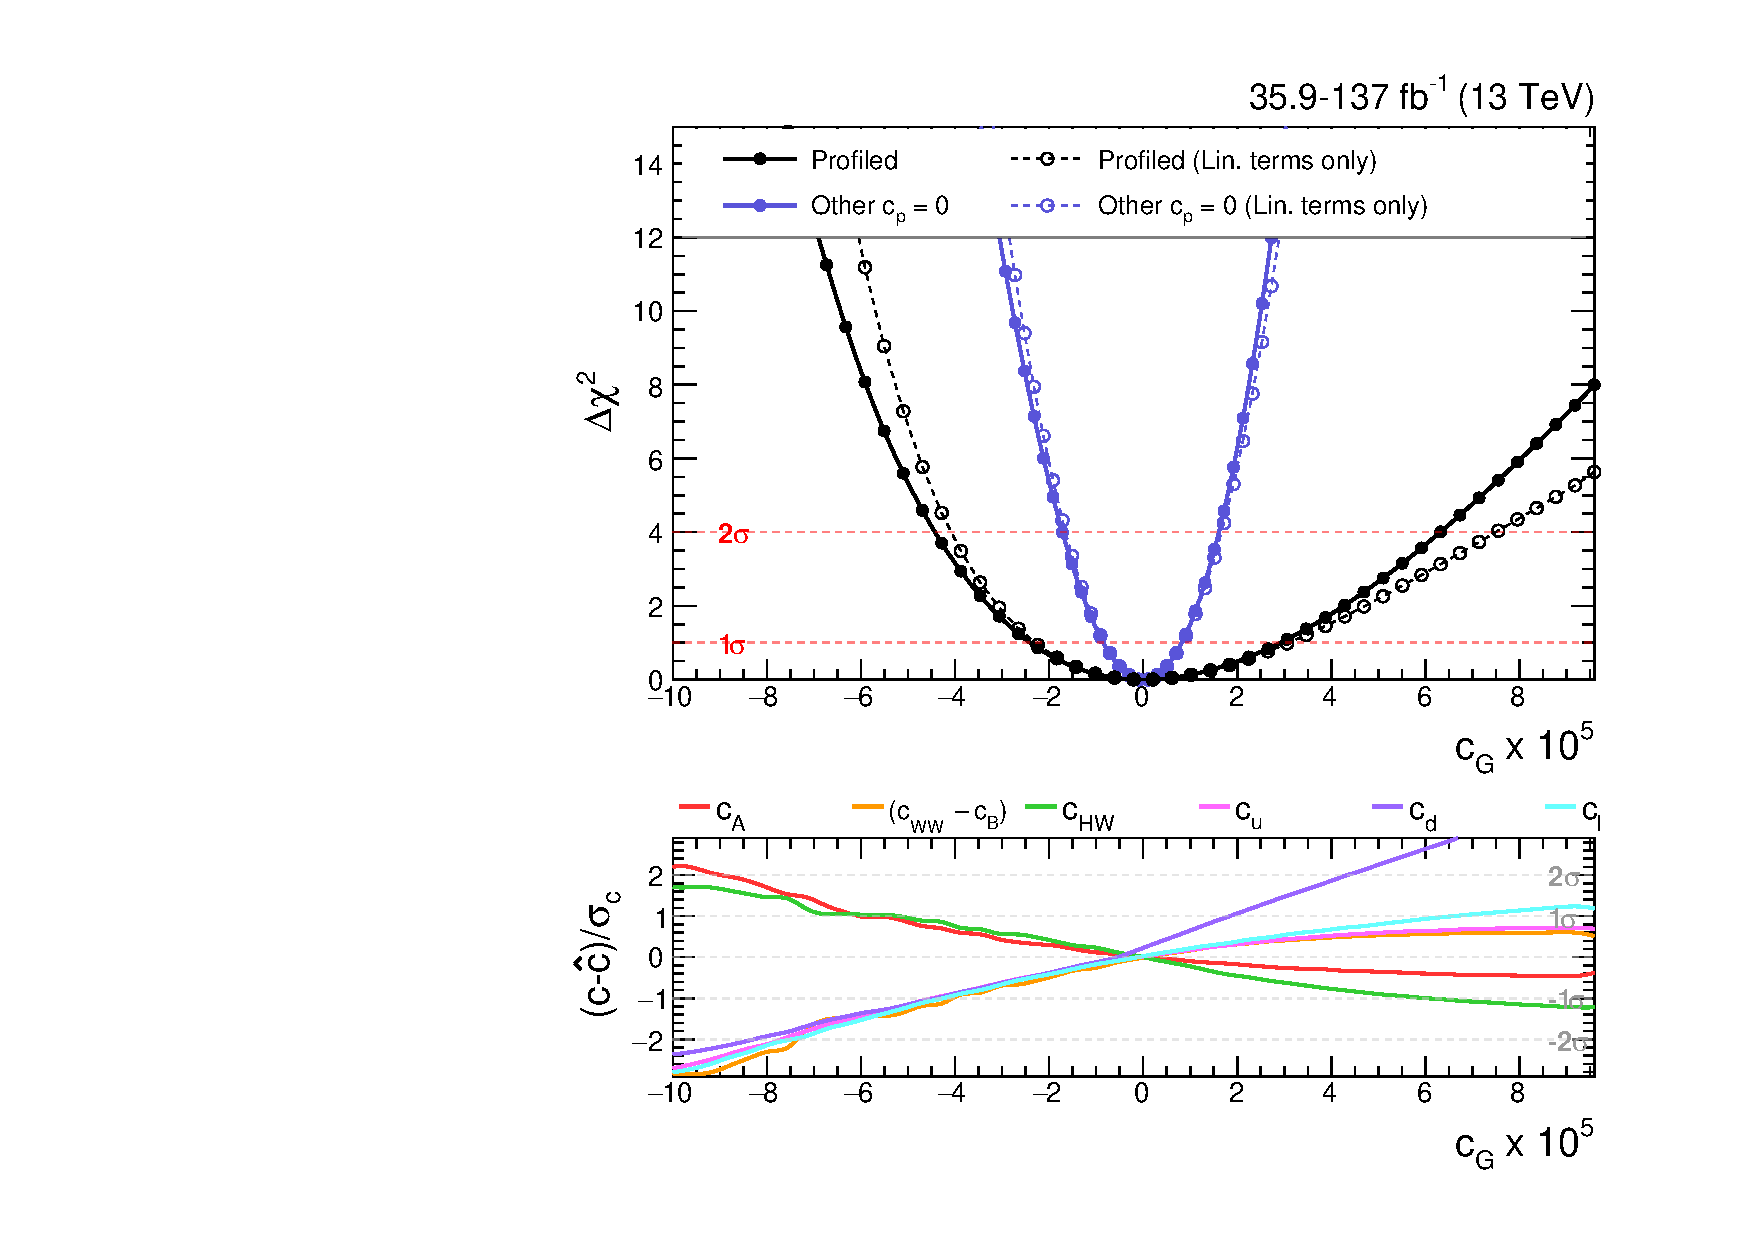
\includegraphics[width=.49\textwidth]{Figures/eft/chi2/expected/cG.pdf}
  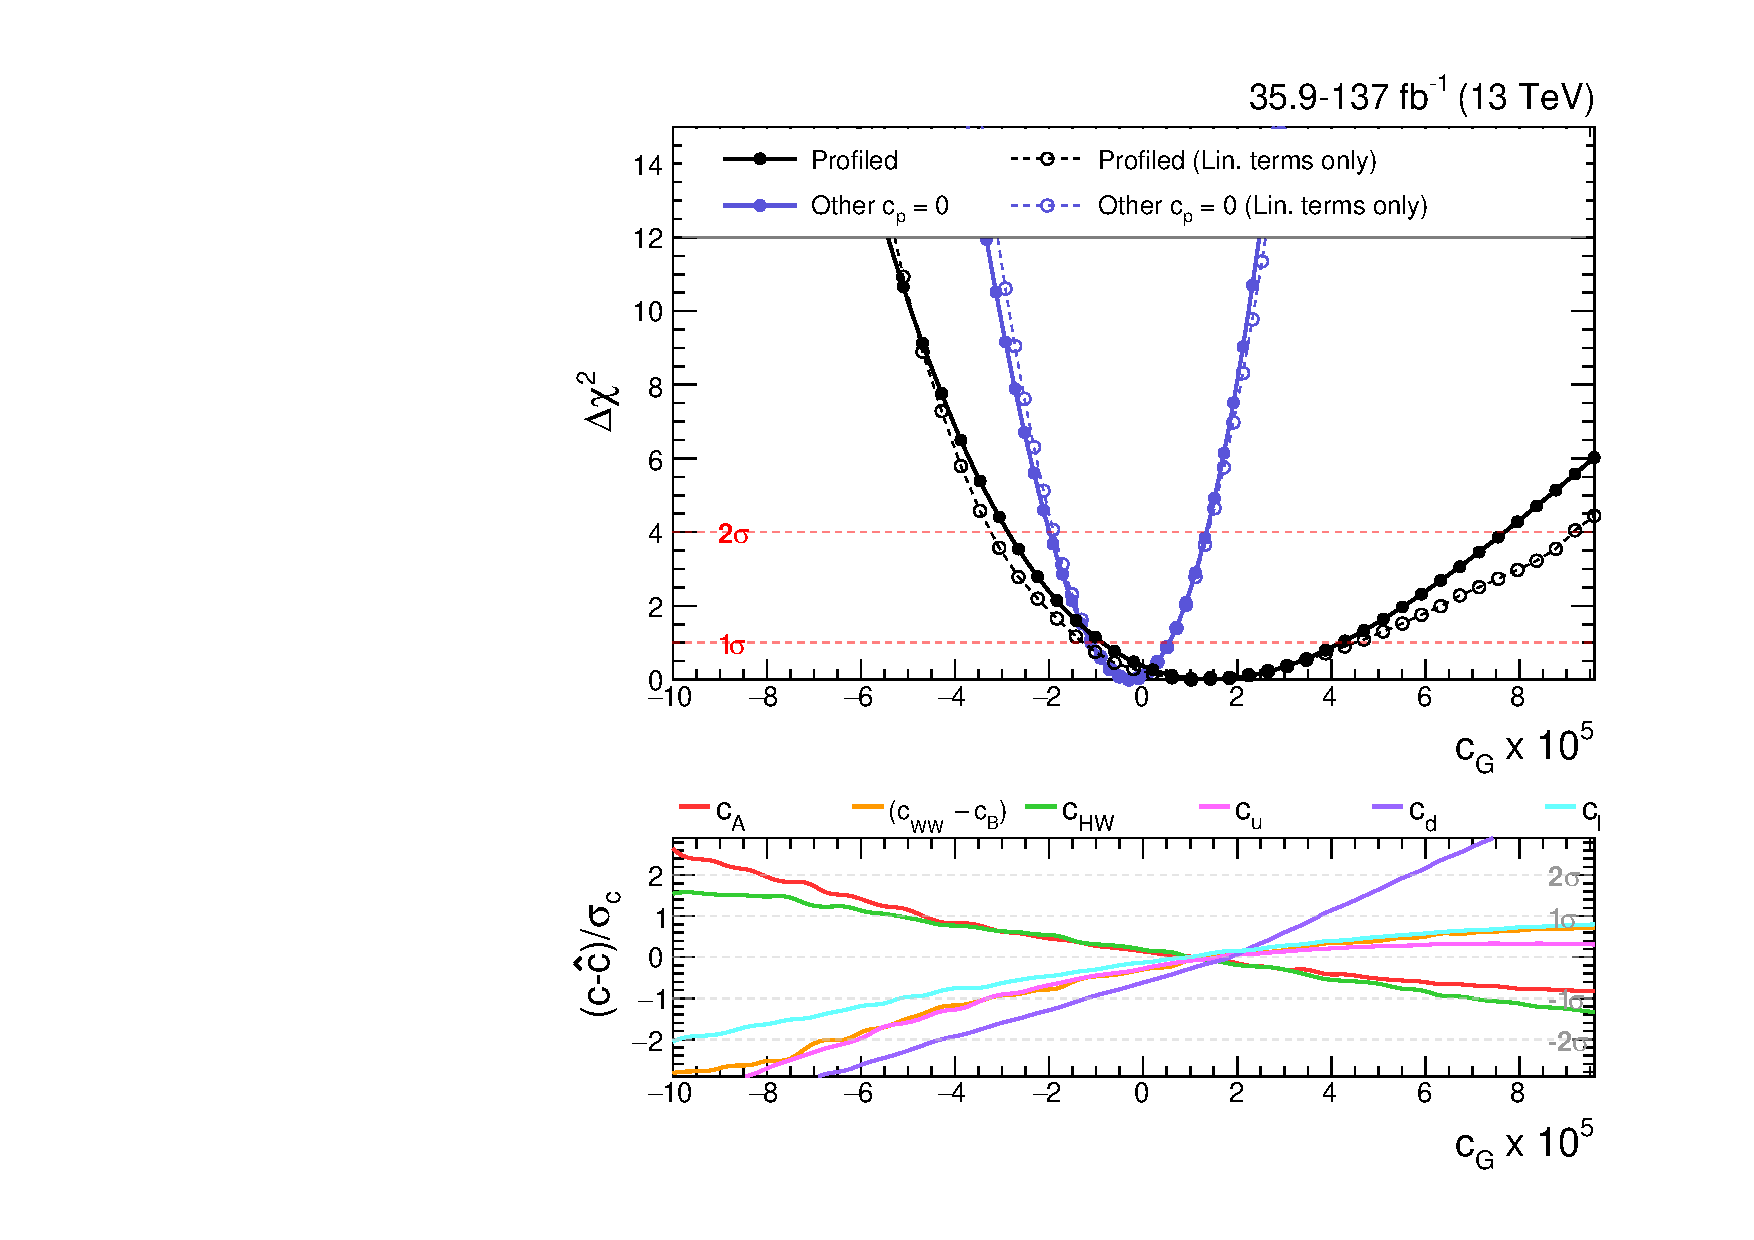
\includegraphics[width=.49\textwidth]{Figures/eft/chi2/observed/cG.pdf}
%   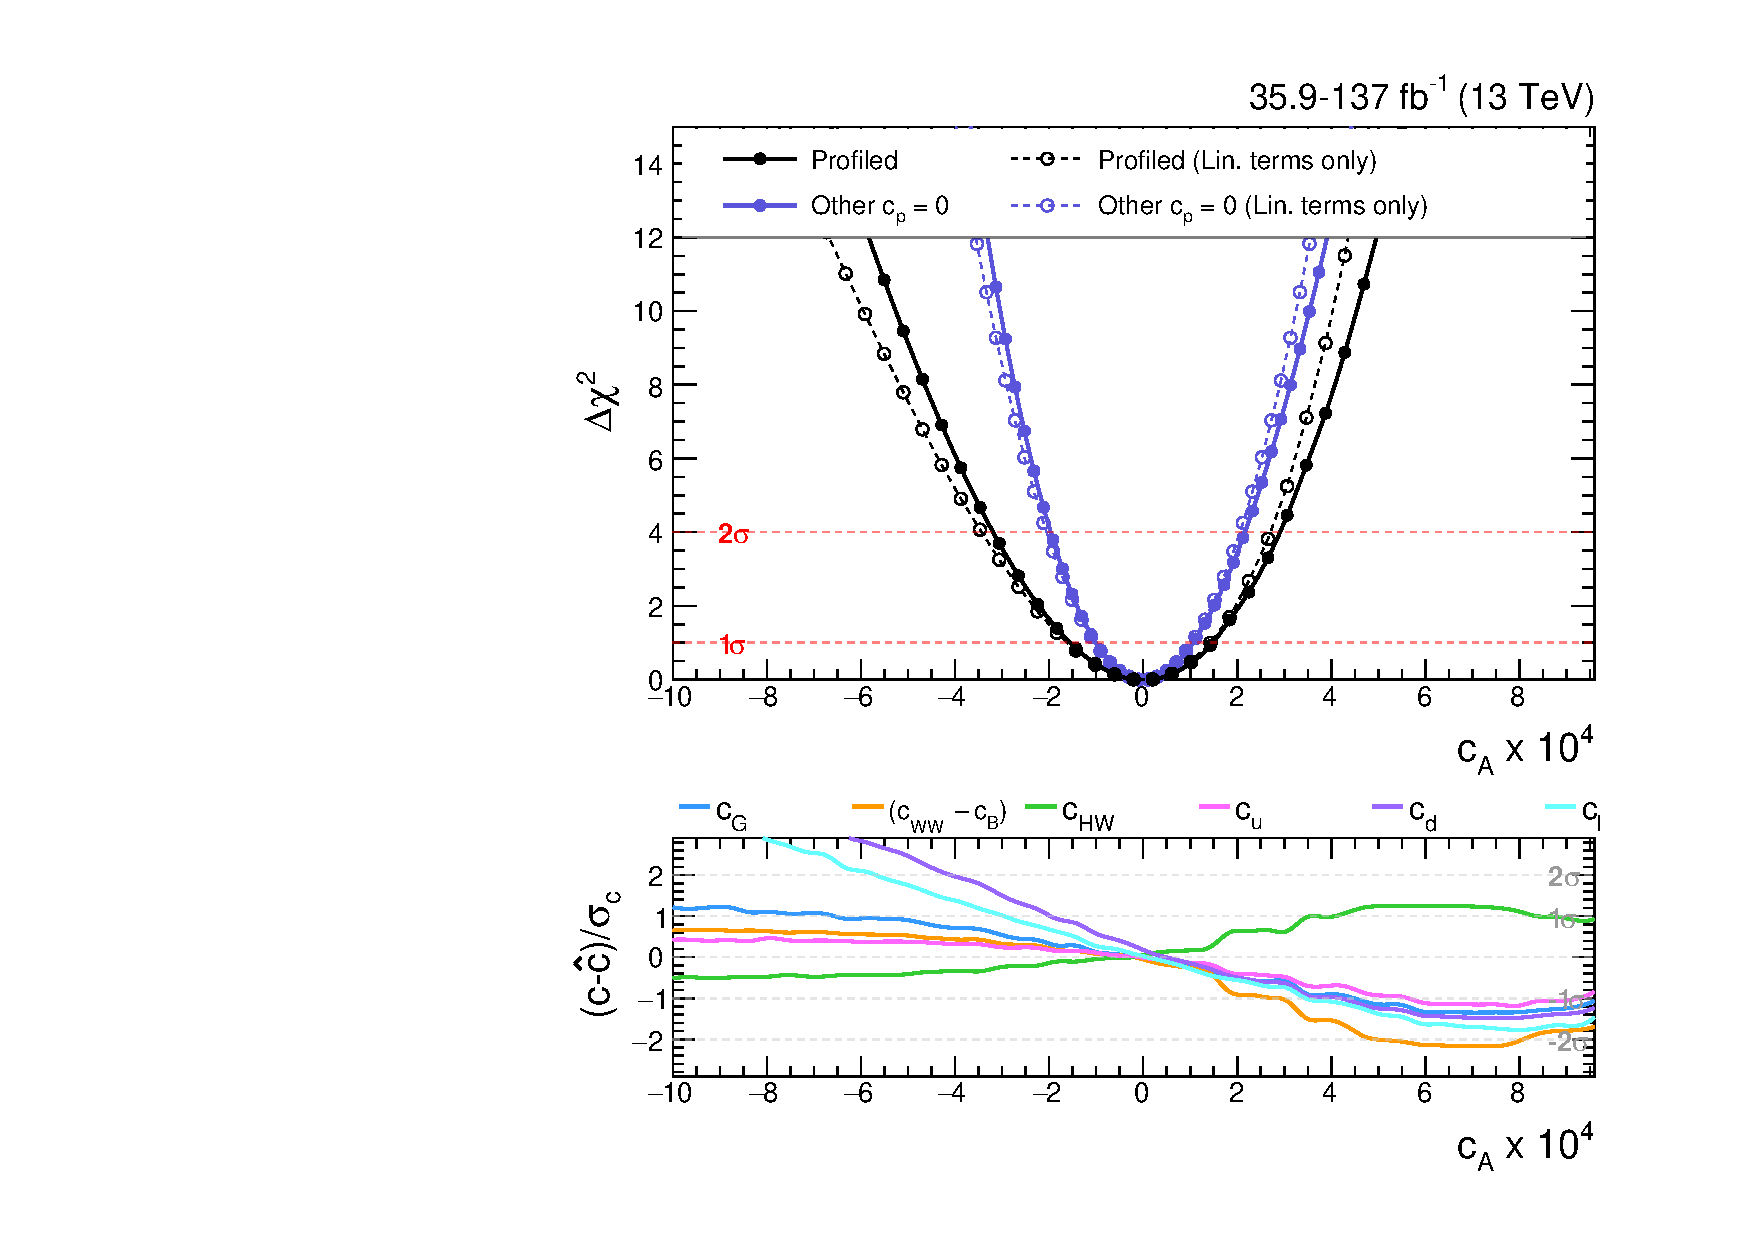
\includegraphics[width=.49\textwidth]{Figures/eft/chi2/expected/cA.pdf}
  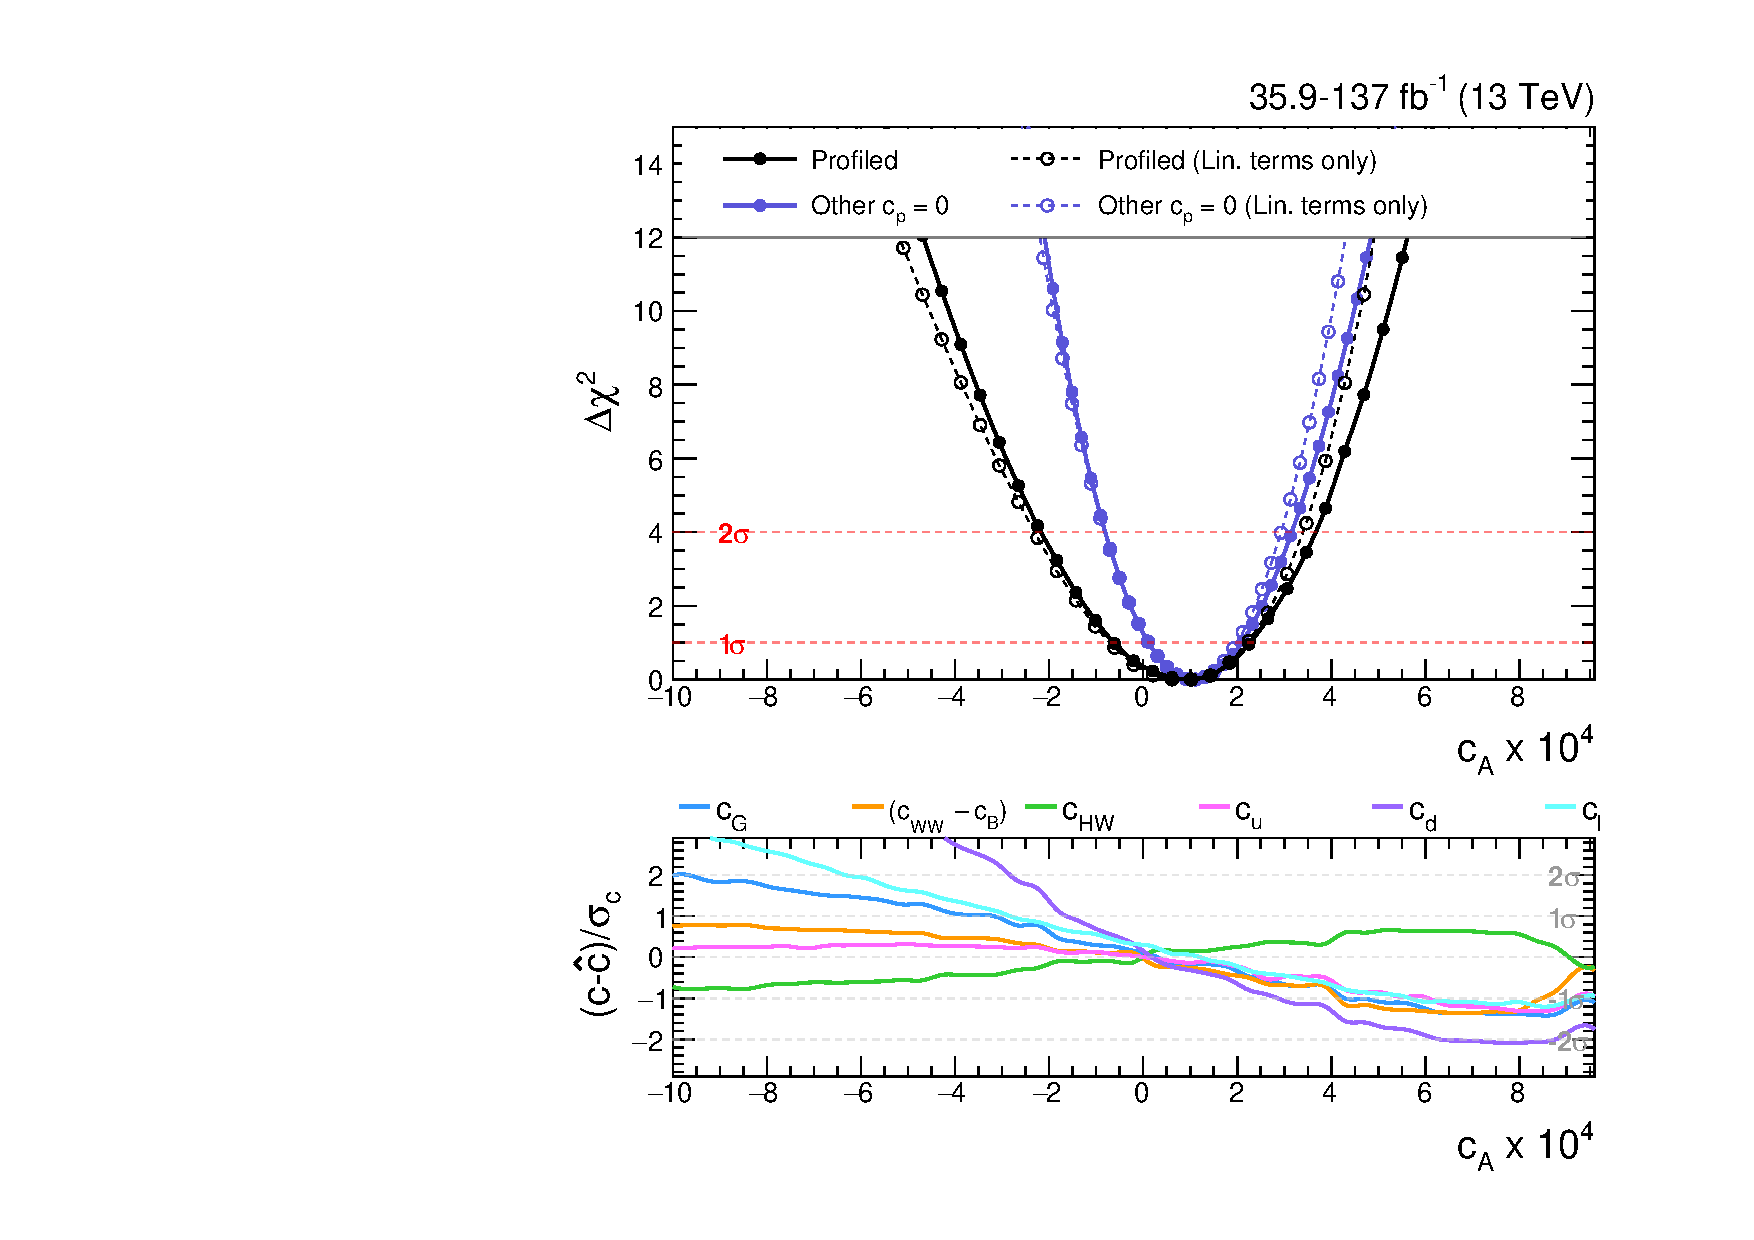
\includegraphics[width=.49\textwidth]{Figures/eft/chi2/observed/cA.pdf}
  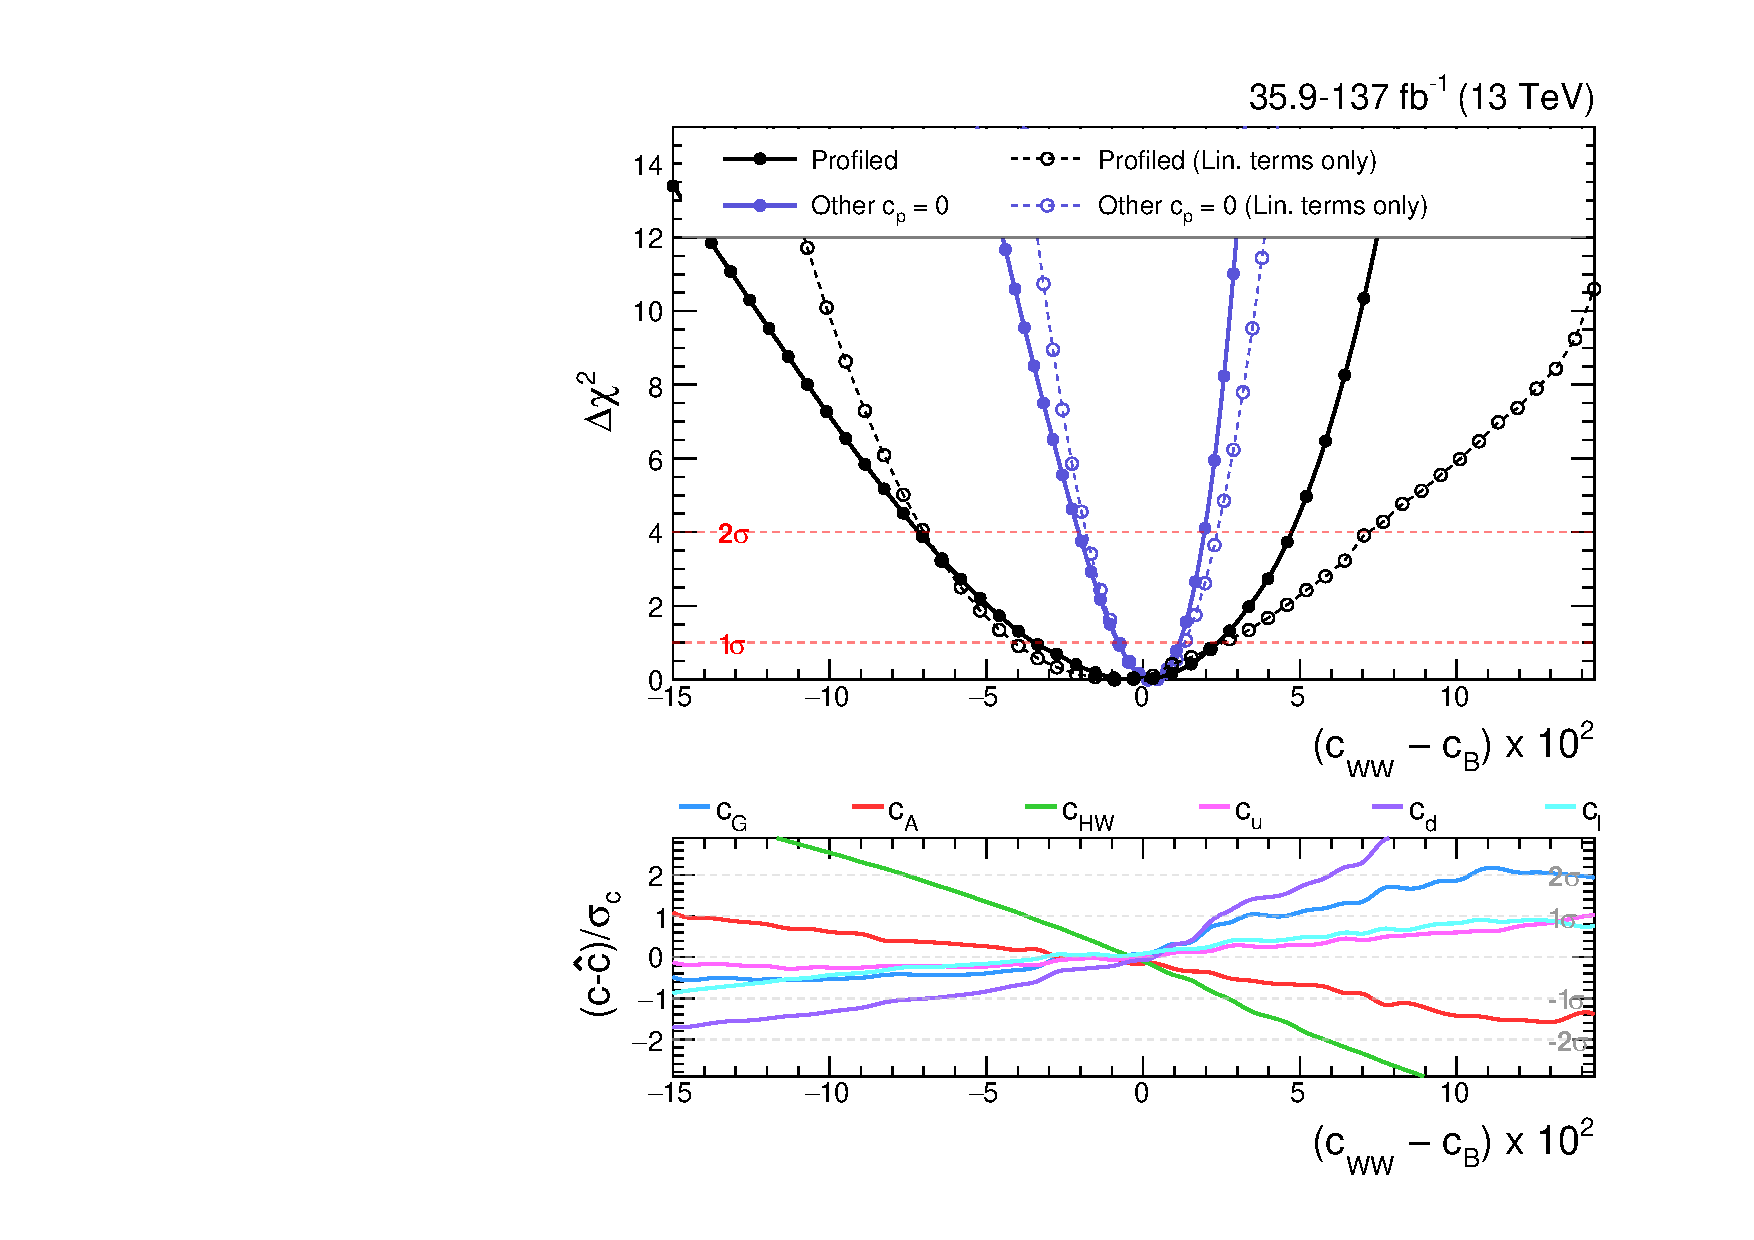
\includegraphics[width=.49\textwidth]{Figures/eft/chi2/observed/cWWMinuscB.pdf}
  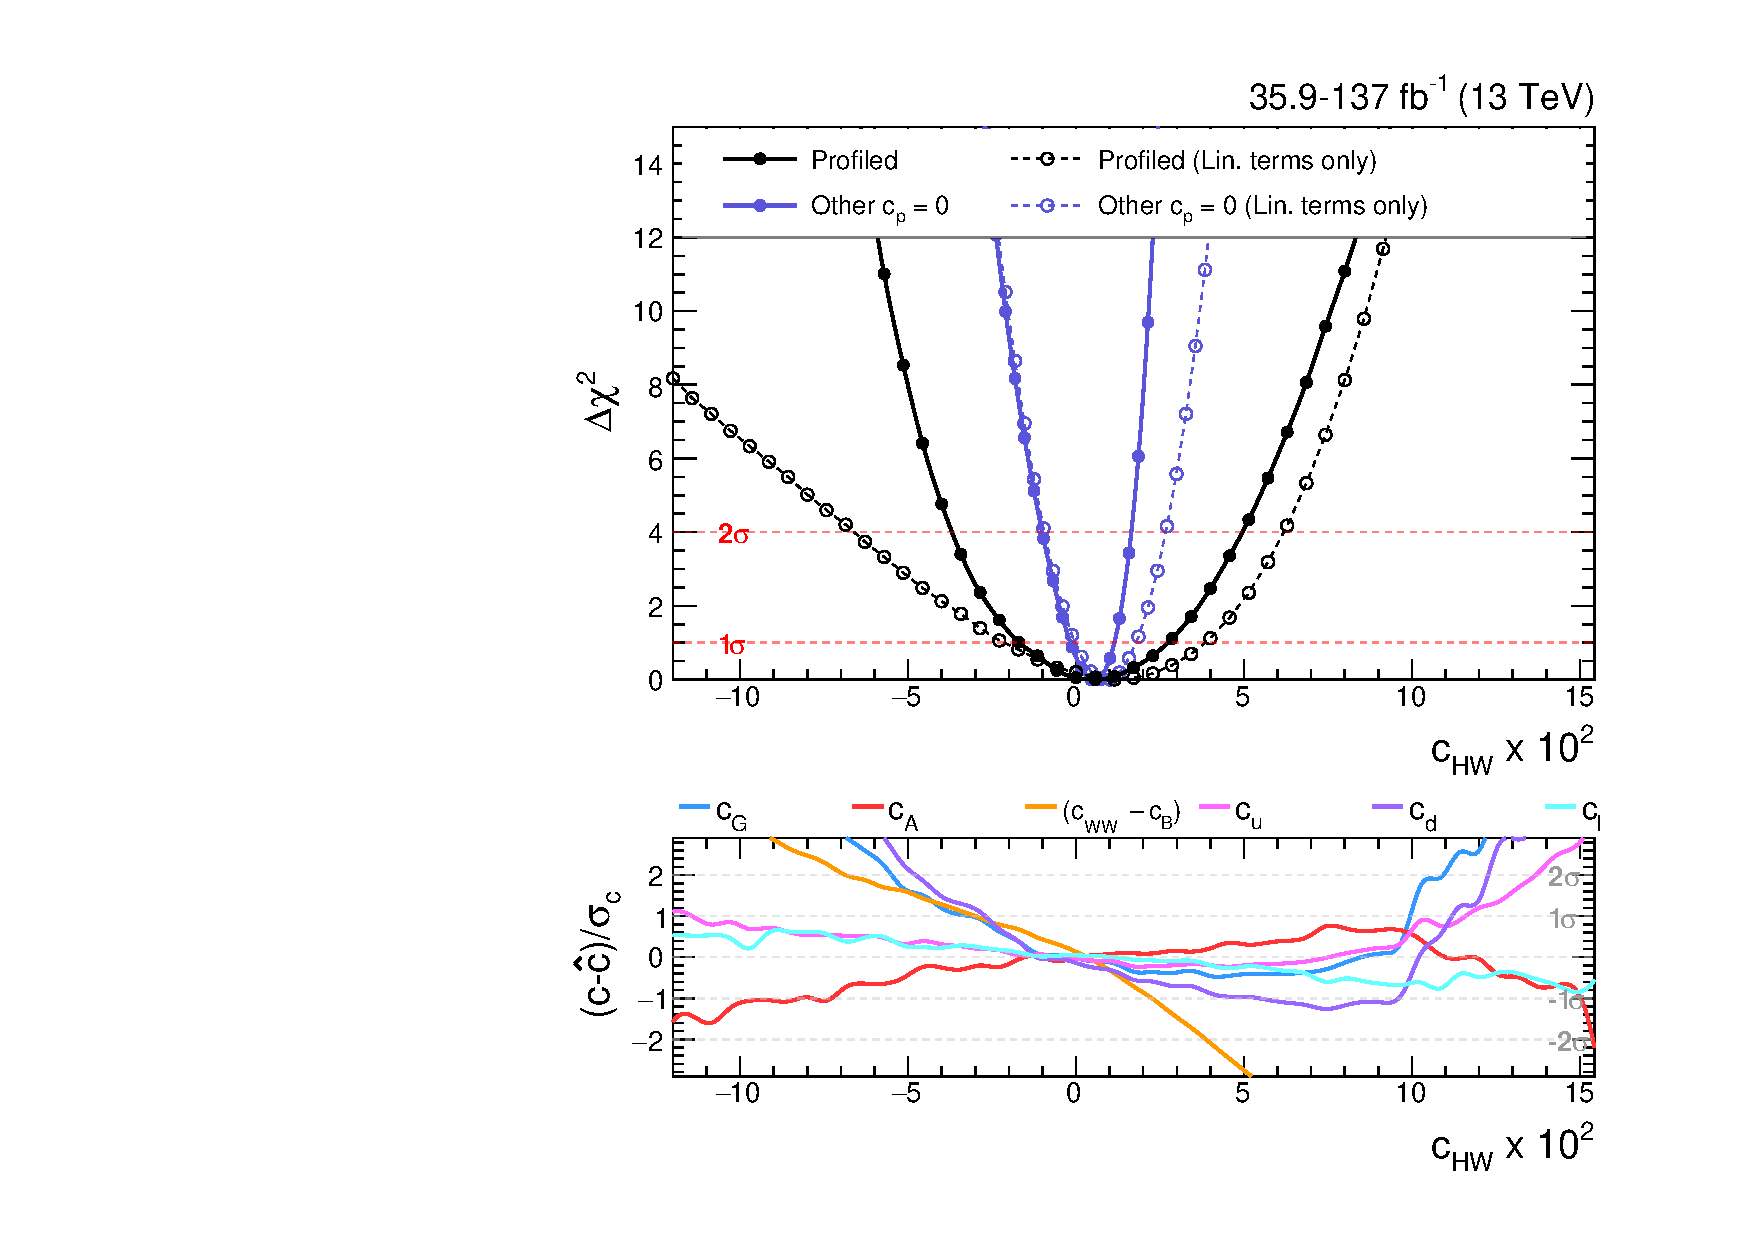
\includegraphics[width=.49\textwidth]{Figures/eft/chi2/observed/cHW.pdf}
  \caption[Simplified HEL re-interpretation: $c_G$, $c_A$, $(c_{WW}-c_B)$ and $c_{HW}$]
  {
    The $\Delta\chi^2(c_p)$ curves for the HEL parameters: $c_G$, $c_A$, $(c_{WW}-c_B)$ and $c_{HW}$. The black and purple in the top panels lines correspond to the fits in which the other parameters are profiled and fixed to the SM, respectively. The dashed lines indicate the fits when only linear terms are considered in the parametrisation. The points in each curve show the values of $c_p$ where the minimisation is performed; the lines are extracted by interpolating between these points. The horizontal red lines at $\Delta\chi^2(c_p)=1$ and 4 indicate the $1\sigma$ and $2\sigma$ confidence intervals in $c_p$, respectively. The bottom panels show the pull of the profiled parameters with respect to the parameter of interest. 
  }
  \label{fig:hel_chi2_simplified_0}
\end{figure}

% \begin{figure}[htb!]
%   \centering
% %   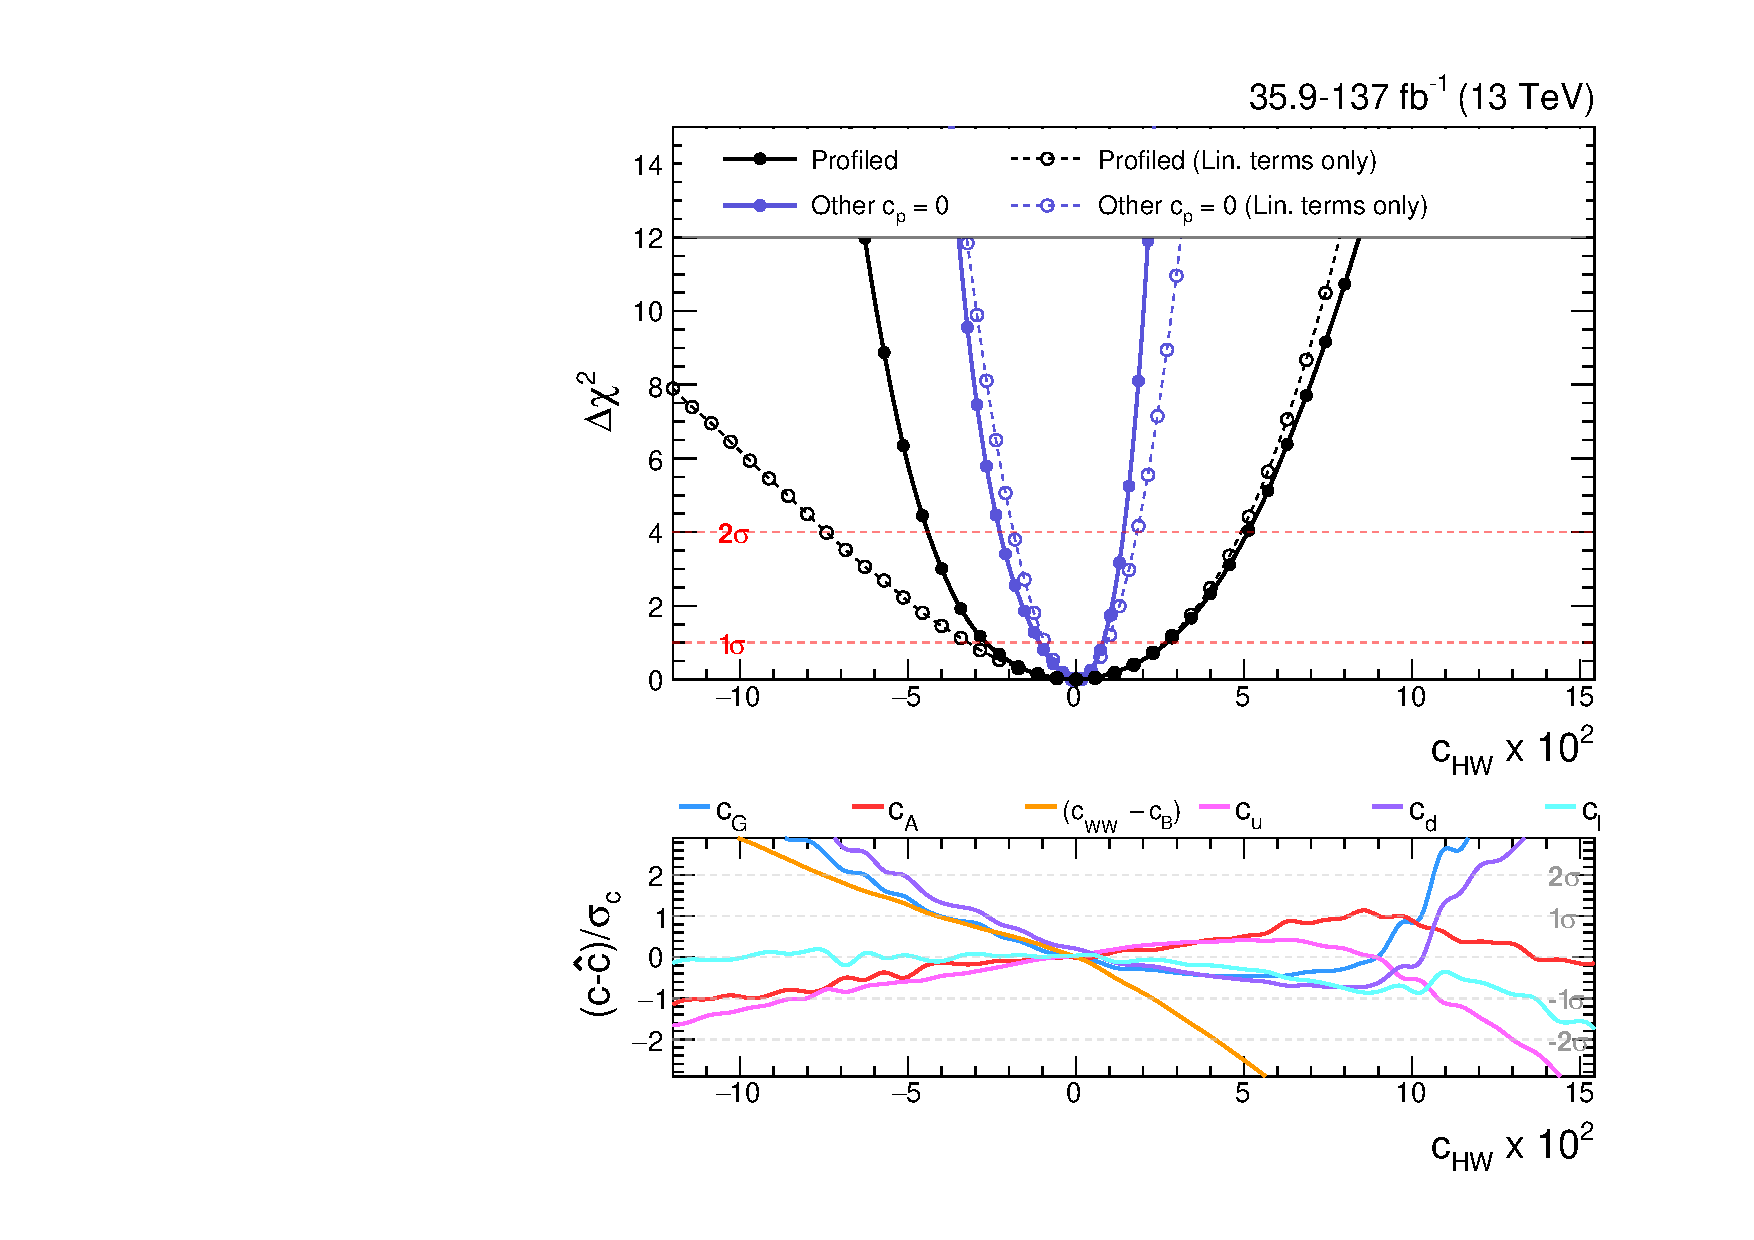
\includegraphics[width=.49\textwidth]{Figures/eft/chi2/expected/cHW.pdf}
% %   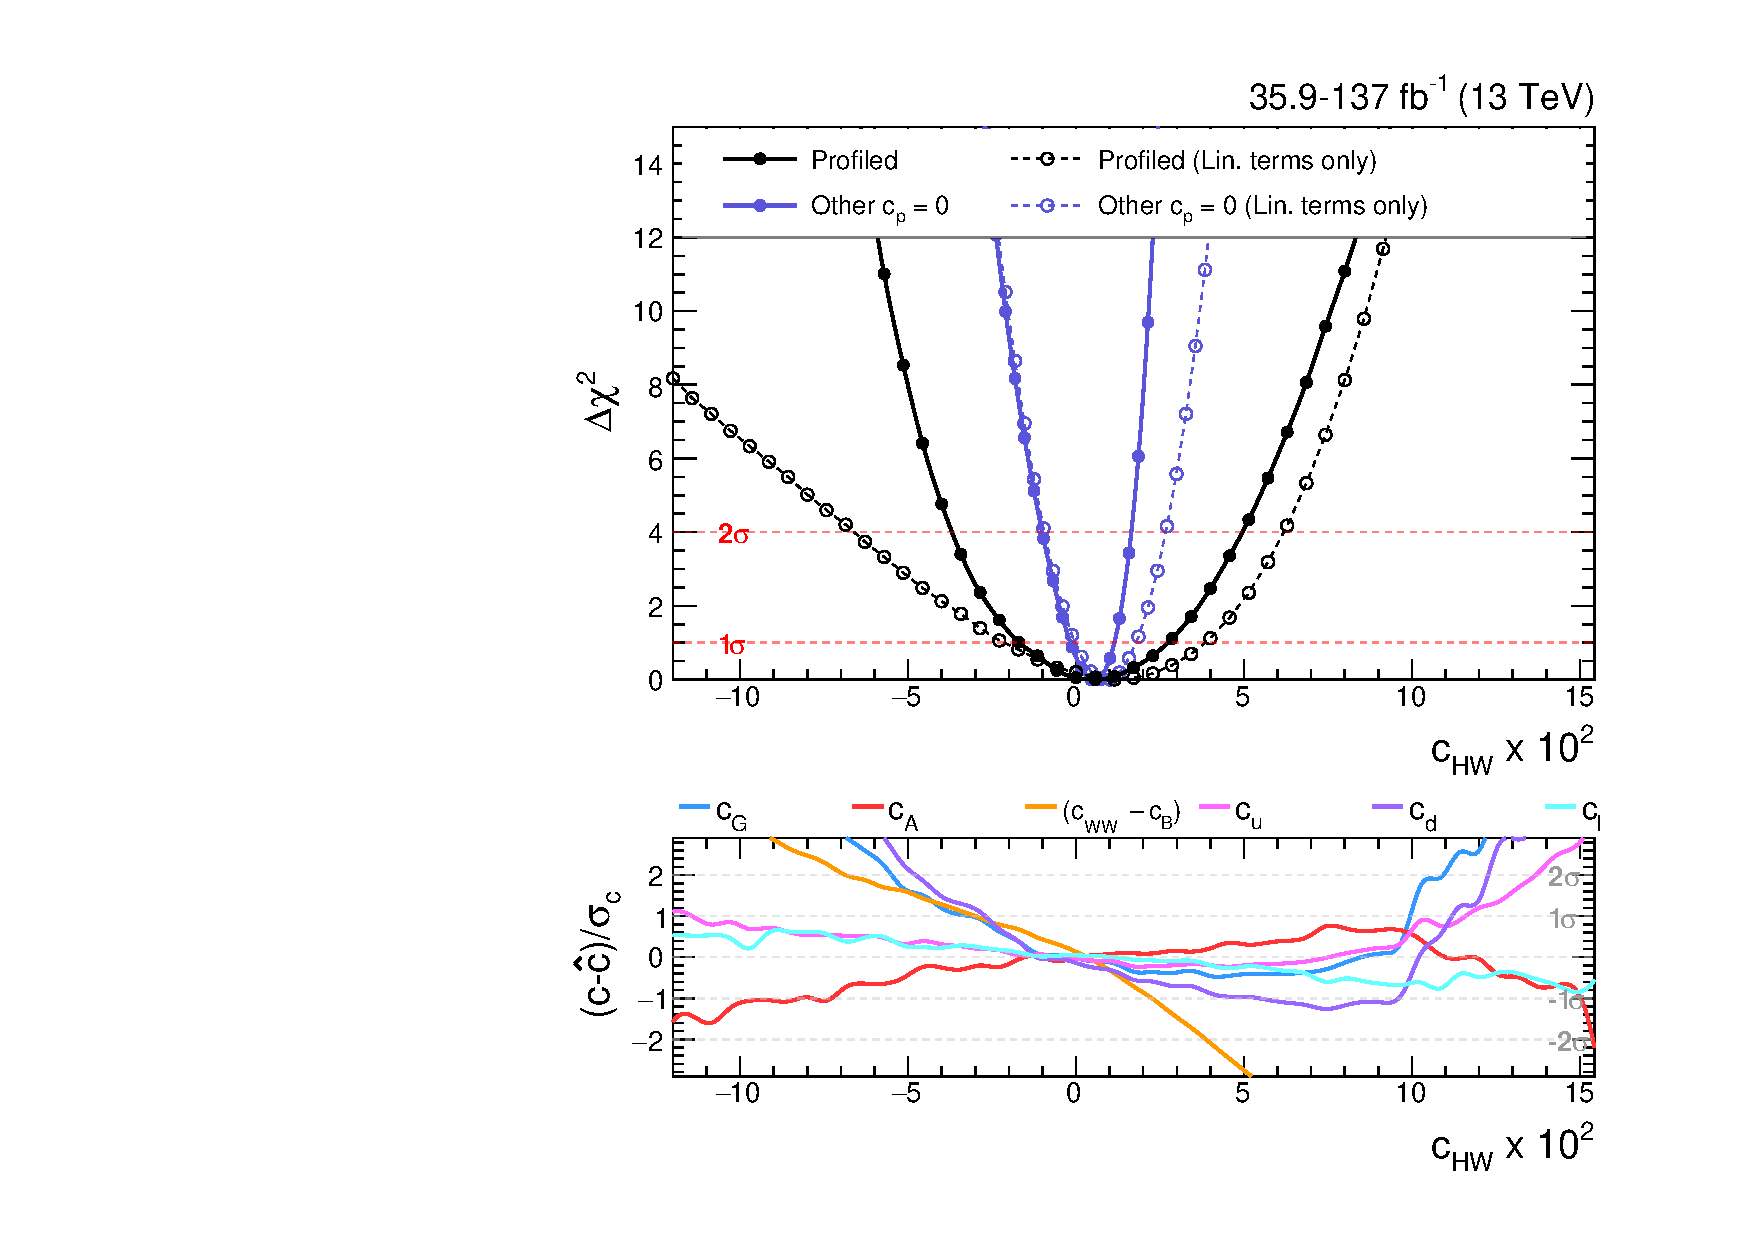
\includegraphics[width=.49\textwidth]{Figures/eft/chi2/observed/cHW.pdf}
% %   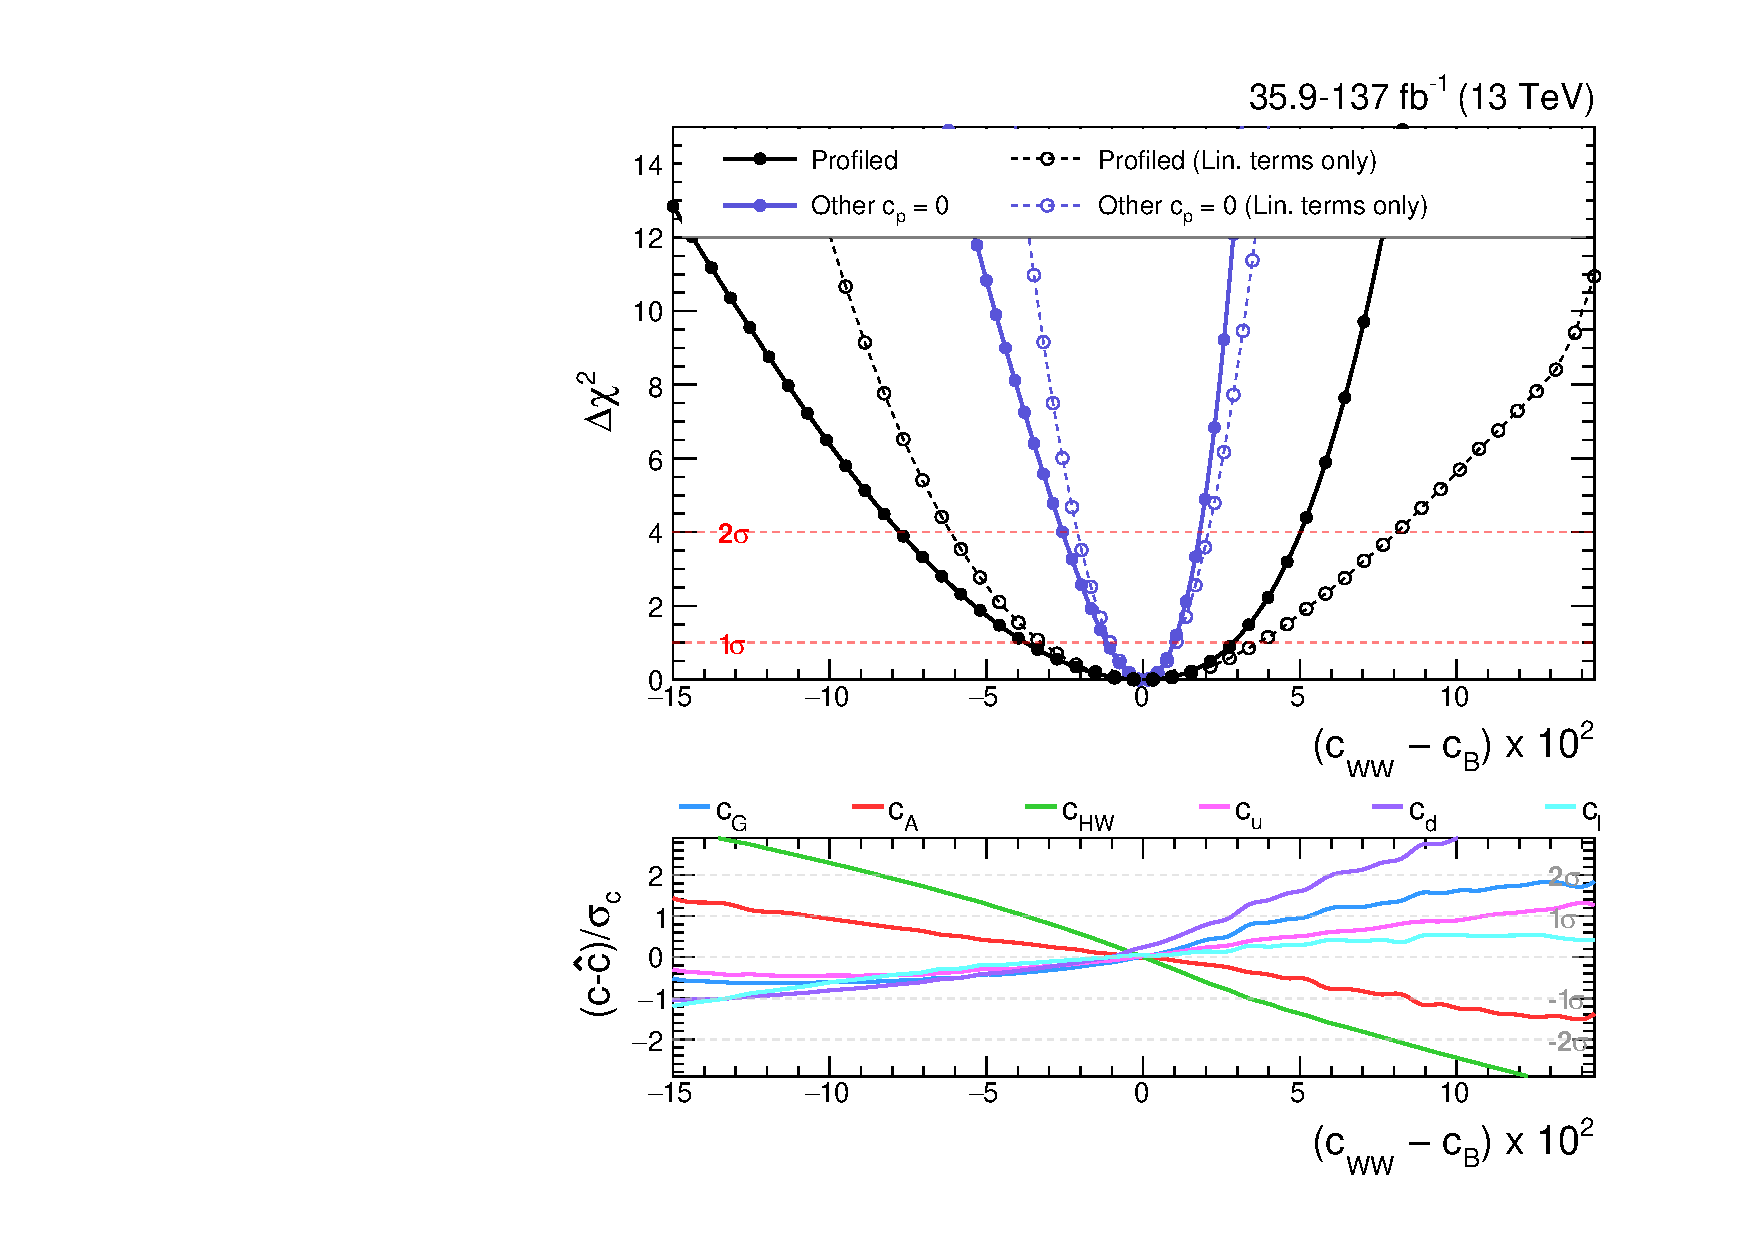
\includegraphics[width=.49\textwidth]{Figures/eft/chi2/expected/cWWMinuscB.pdf}
% %   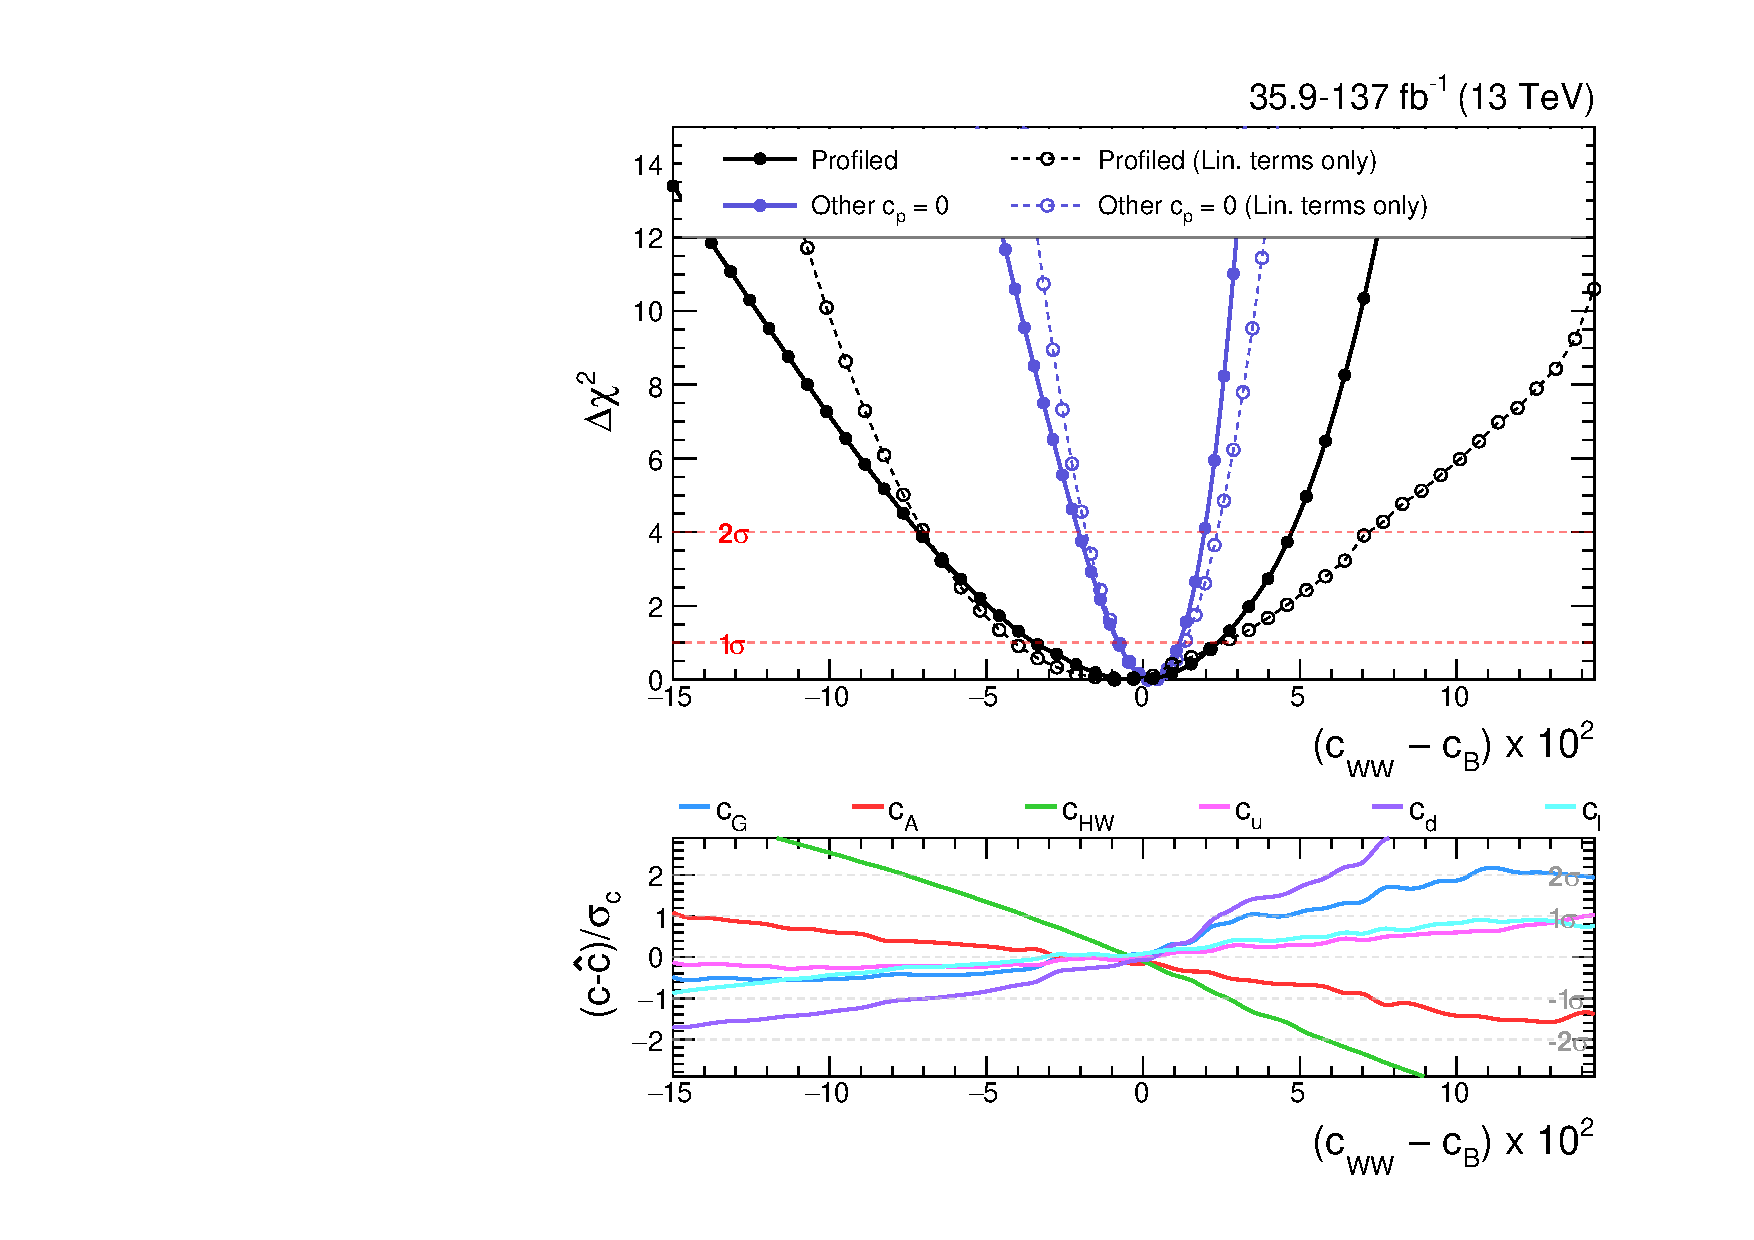
\includegraphics[width=.49\textwidth]{Figures/eft/chi2/observed/cWWMinuscB.pdf}
%   \caption[Simplified HEL re-interpretation: $(c_{WW}-c_B)$ and $c_{HW}$]
%   {
%     Add caption
%   }
%   \label{fig:hel_chi2_simplified_1}
% \end{figure}

\begin{figure}[htb!]
  \centering
%   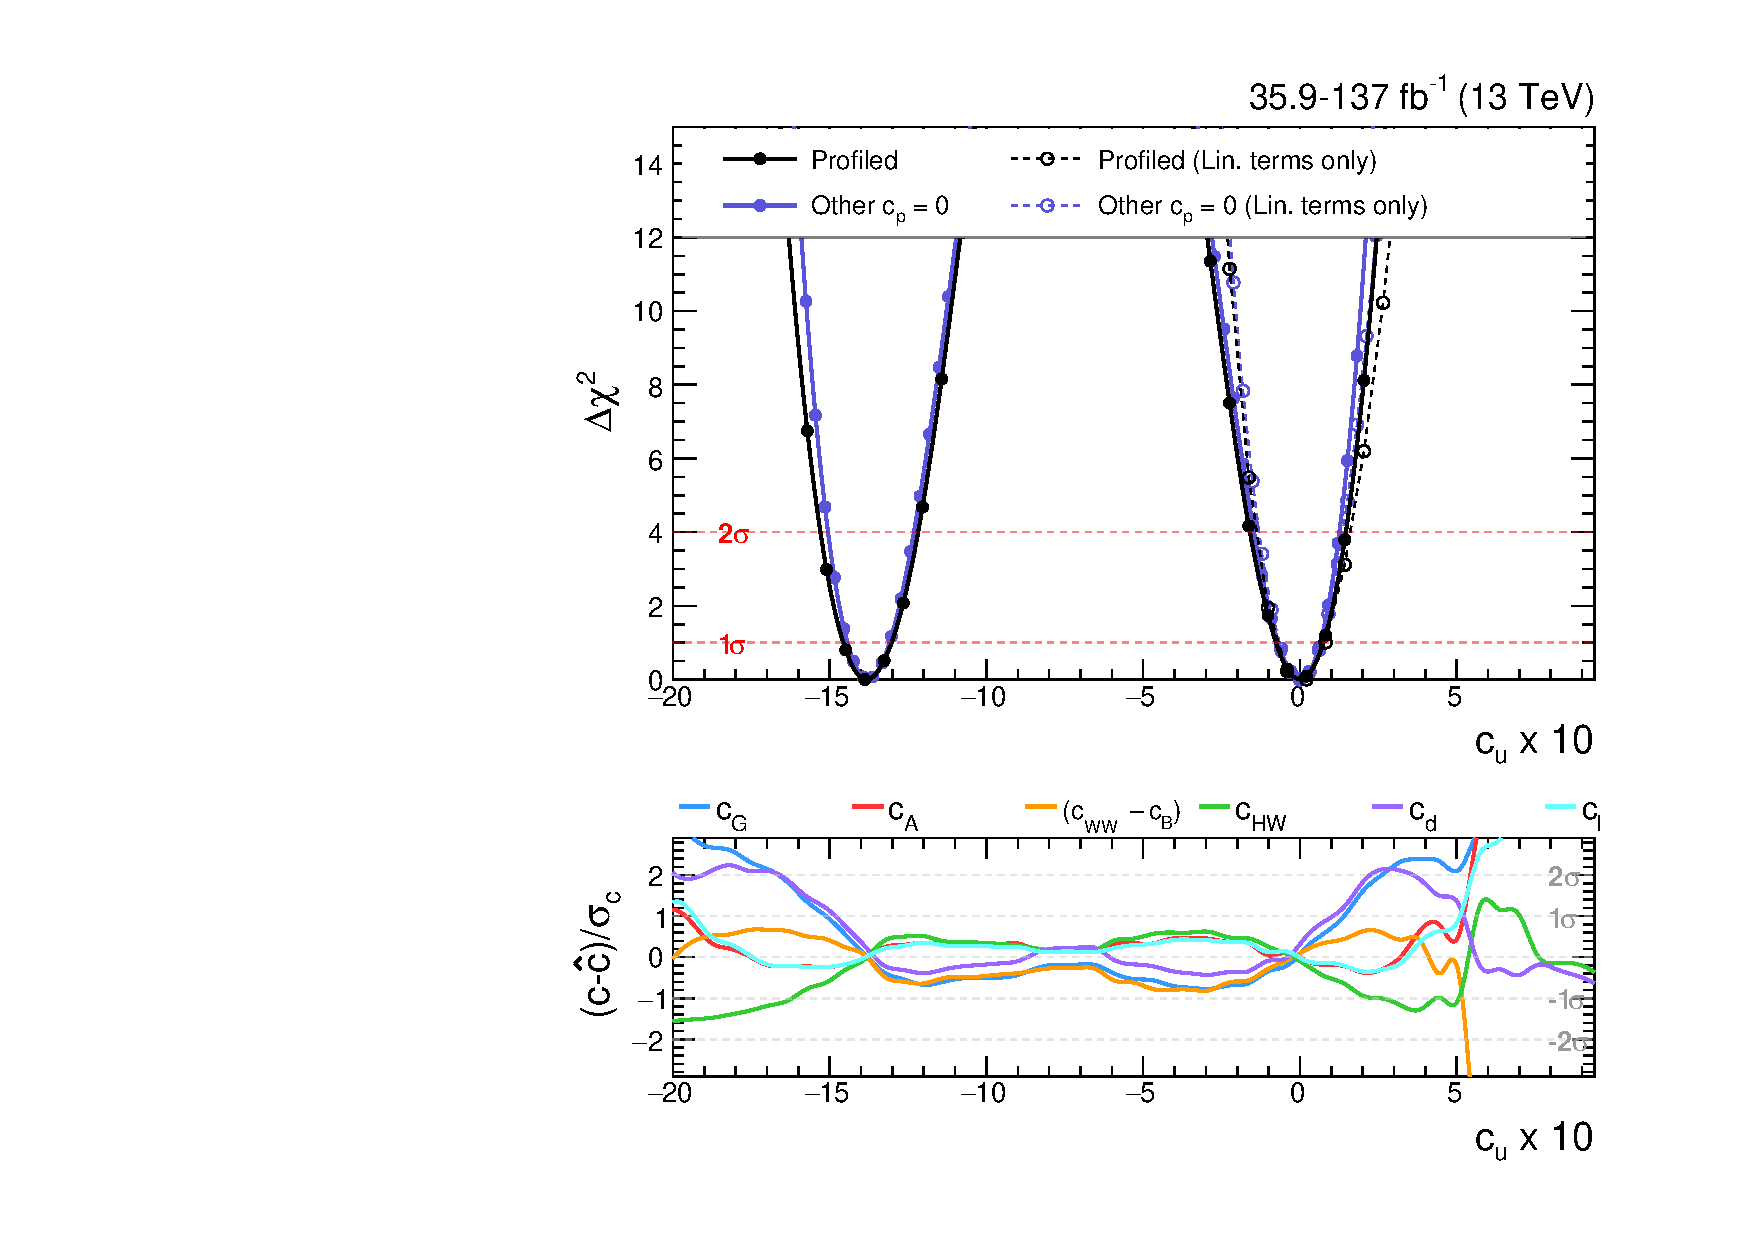
\includegraphics[width=.49\textwidth]{Figures/eft/chi2/expected/cu.pdf}
  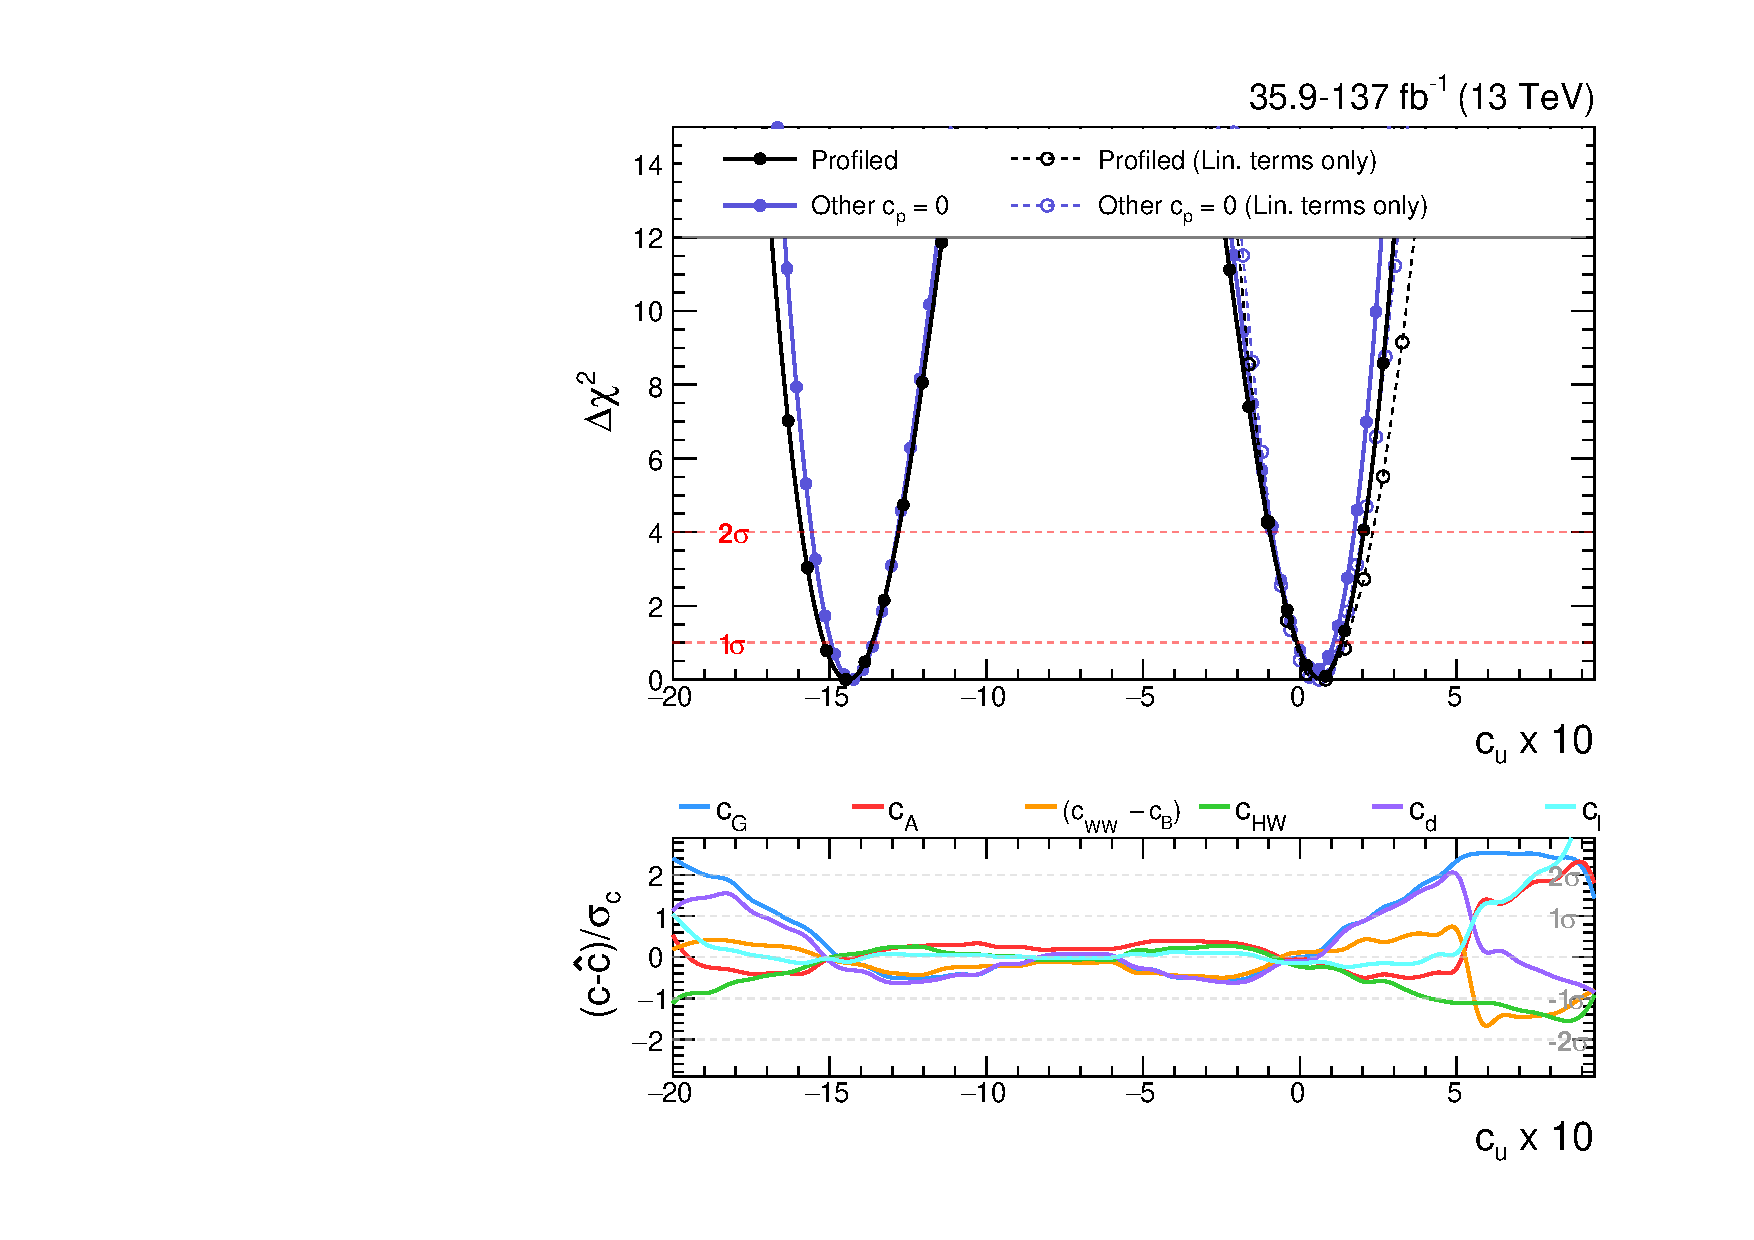
\includegraphics[width=.49\textwidth]{Figures/eft/chi2/observed/cu.pdf}
%   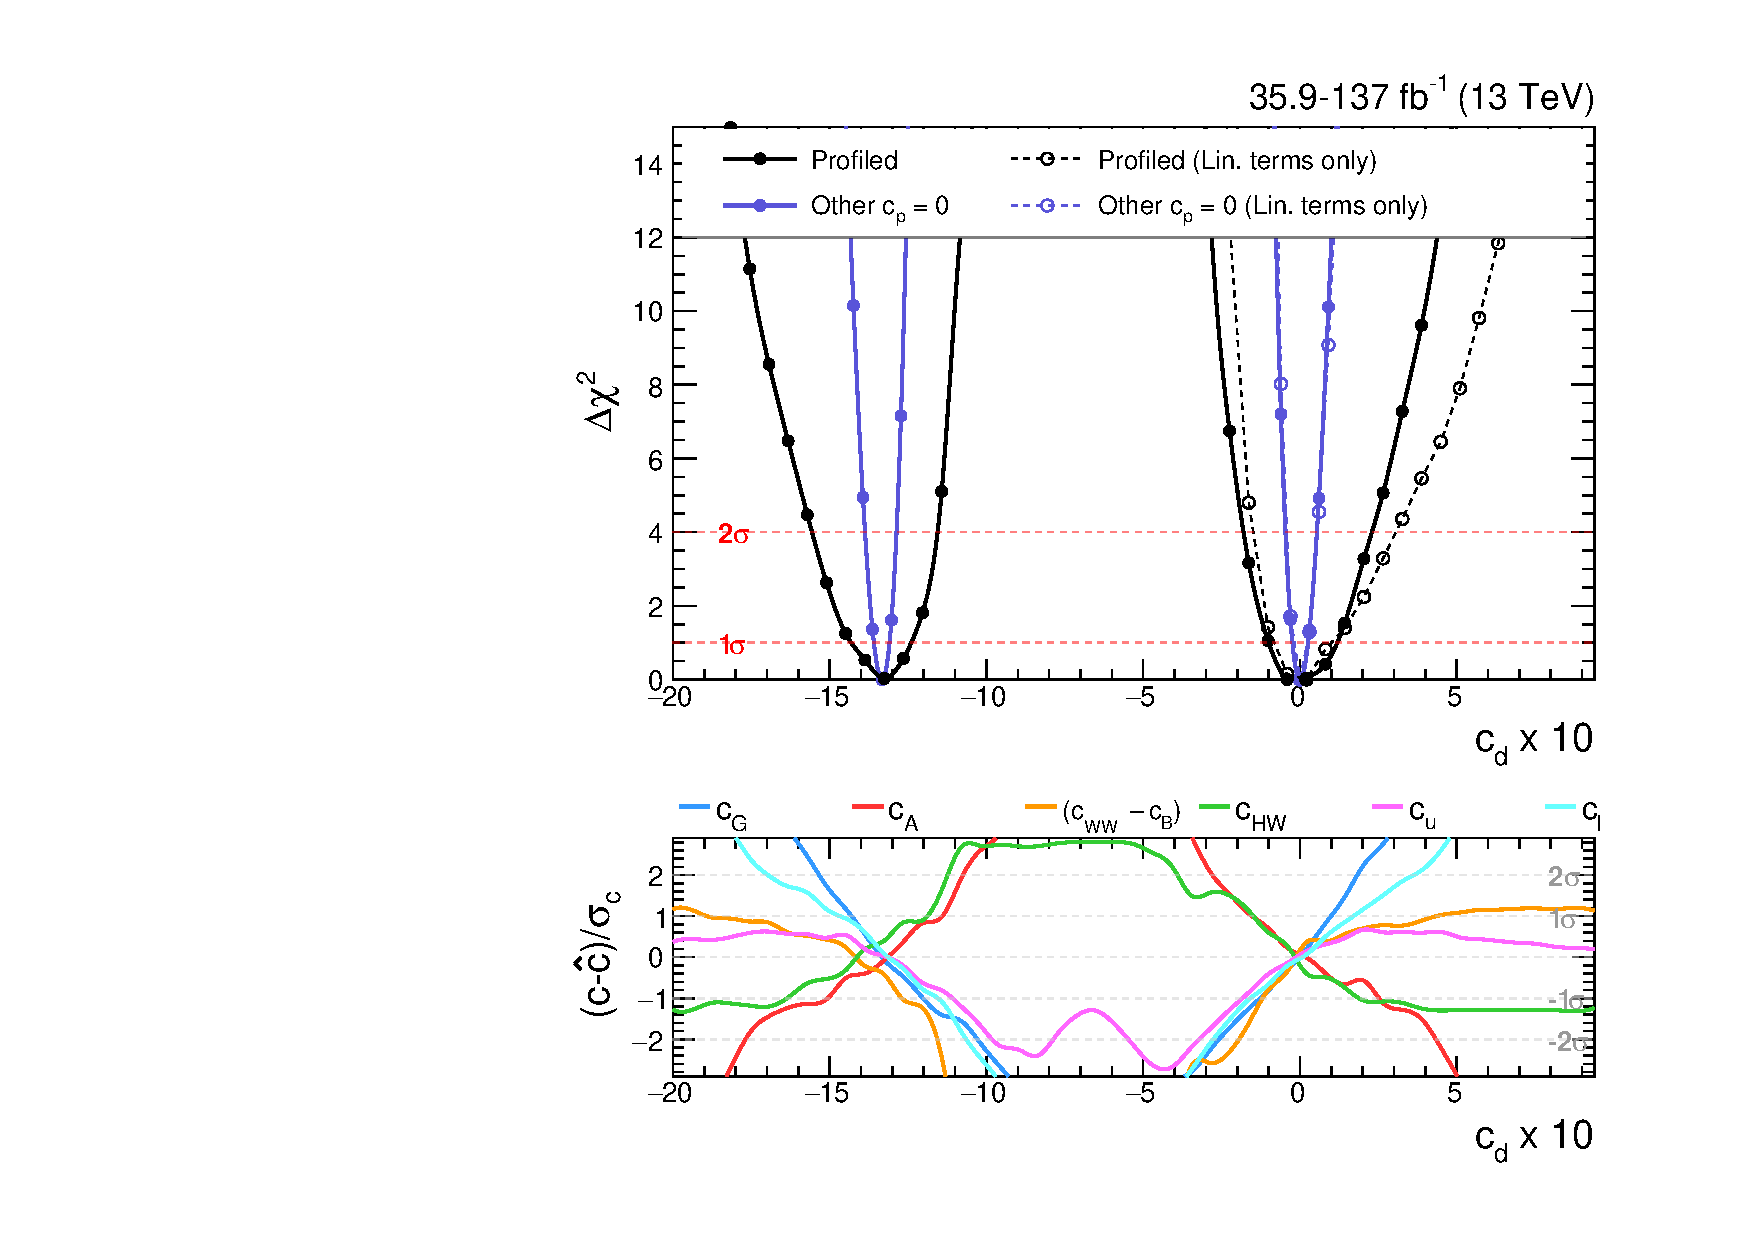
\includegraphics[width=.49\textwidth]{Figures/eft/chi2/expected/cd.pdf}
  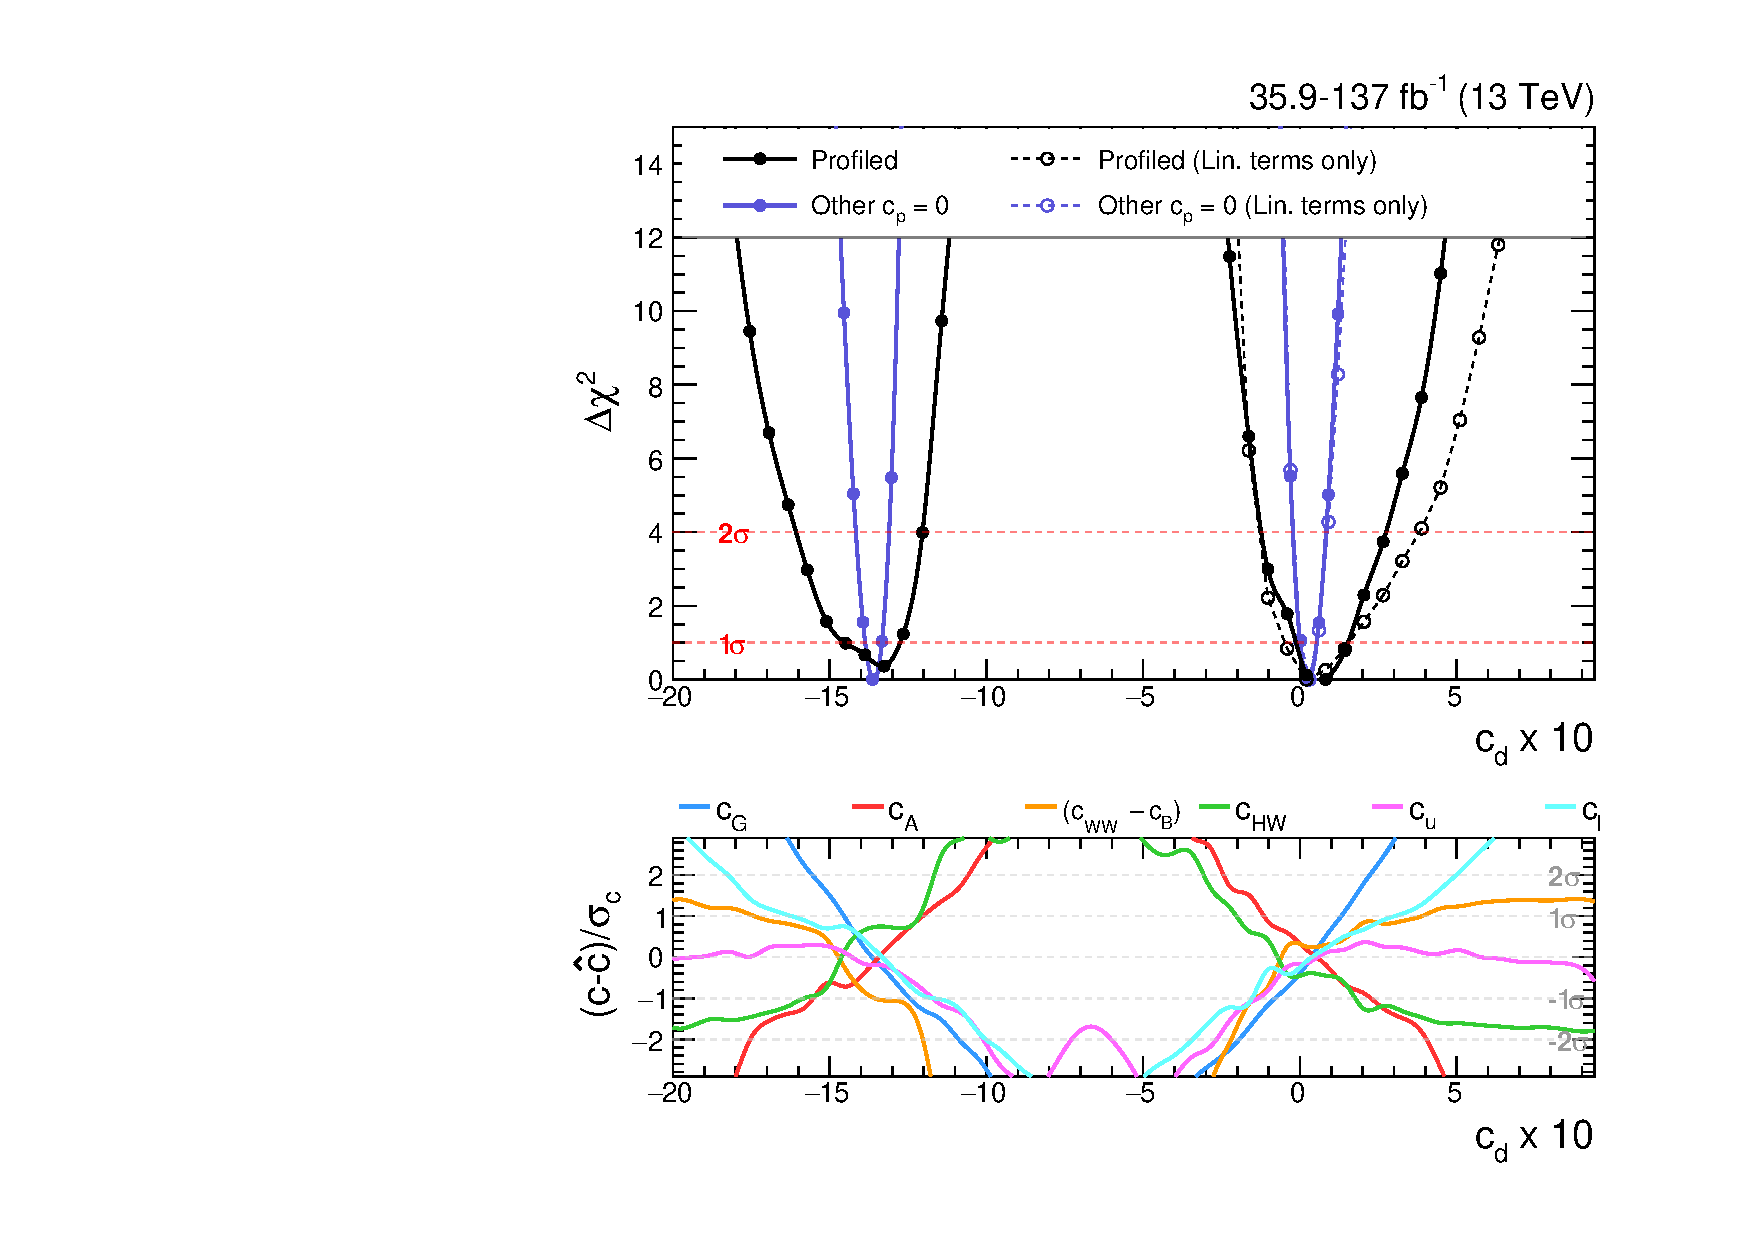
\includegraphics[width=.49\textwidth]{Figures/eft/chi2/observed/cd.pdf}
%   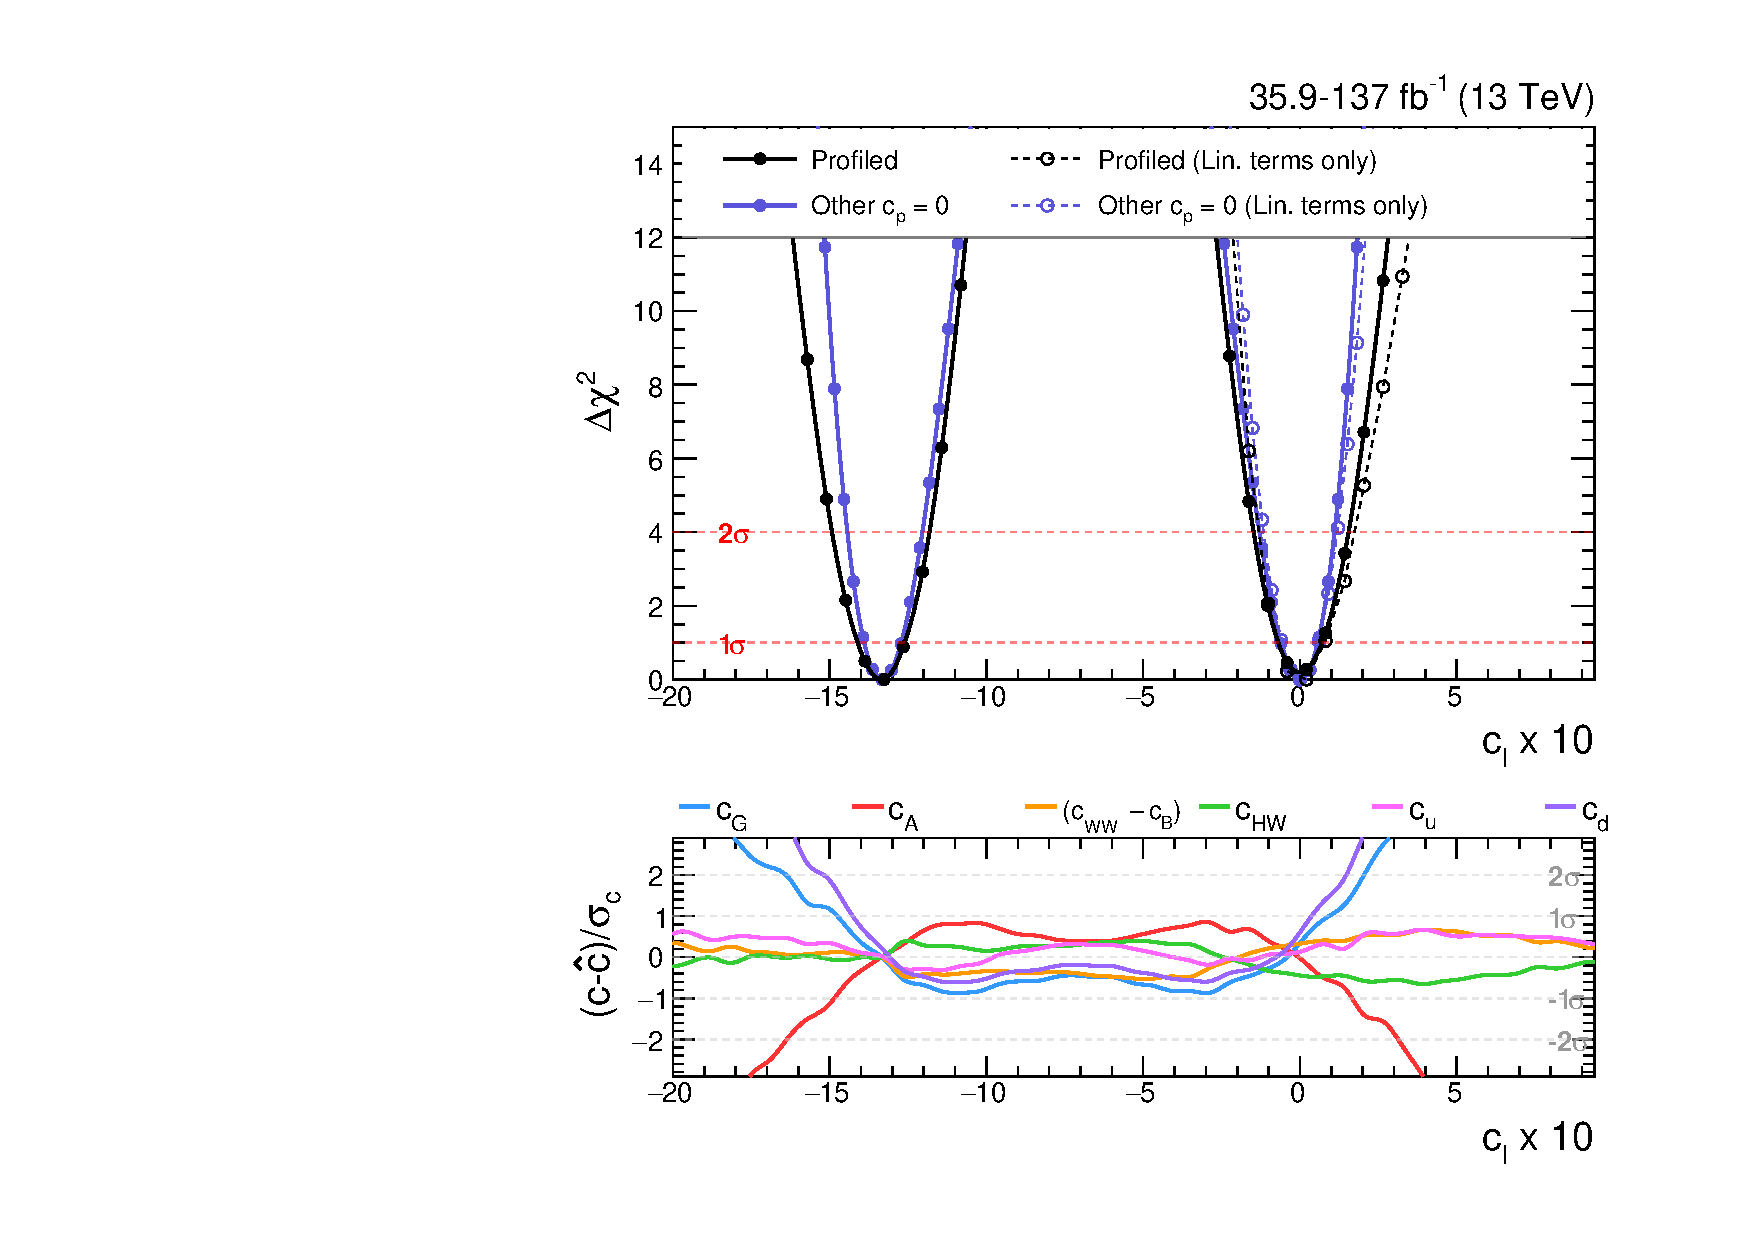
\includegraphics[width=.49\textwidth]{Figures/eft/chi2/expected/cl.pdf}
  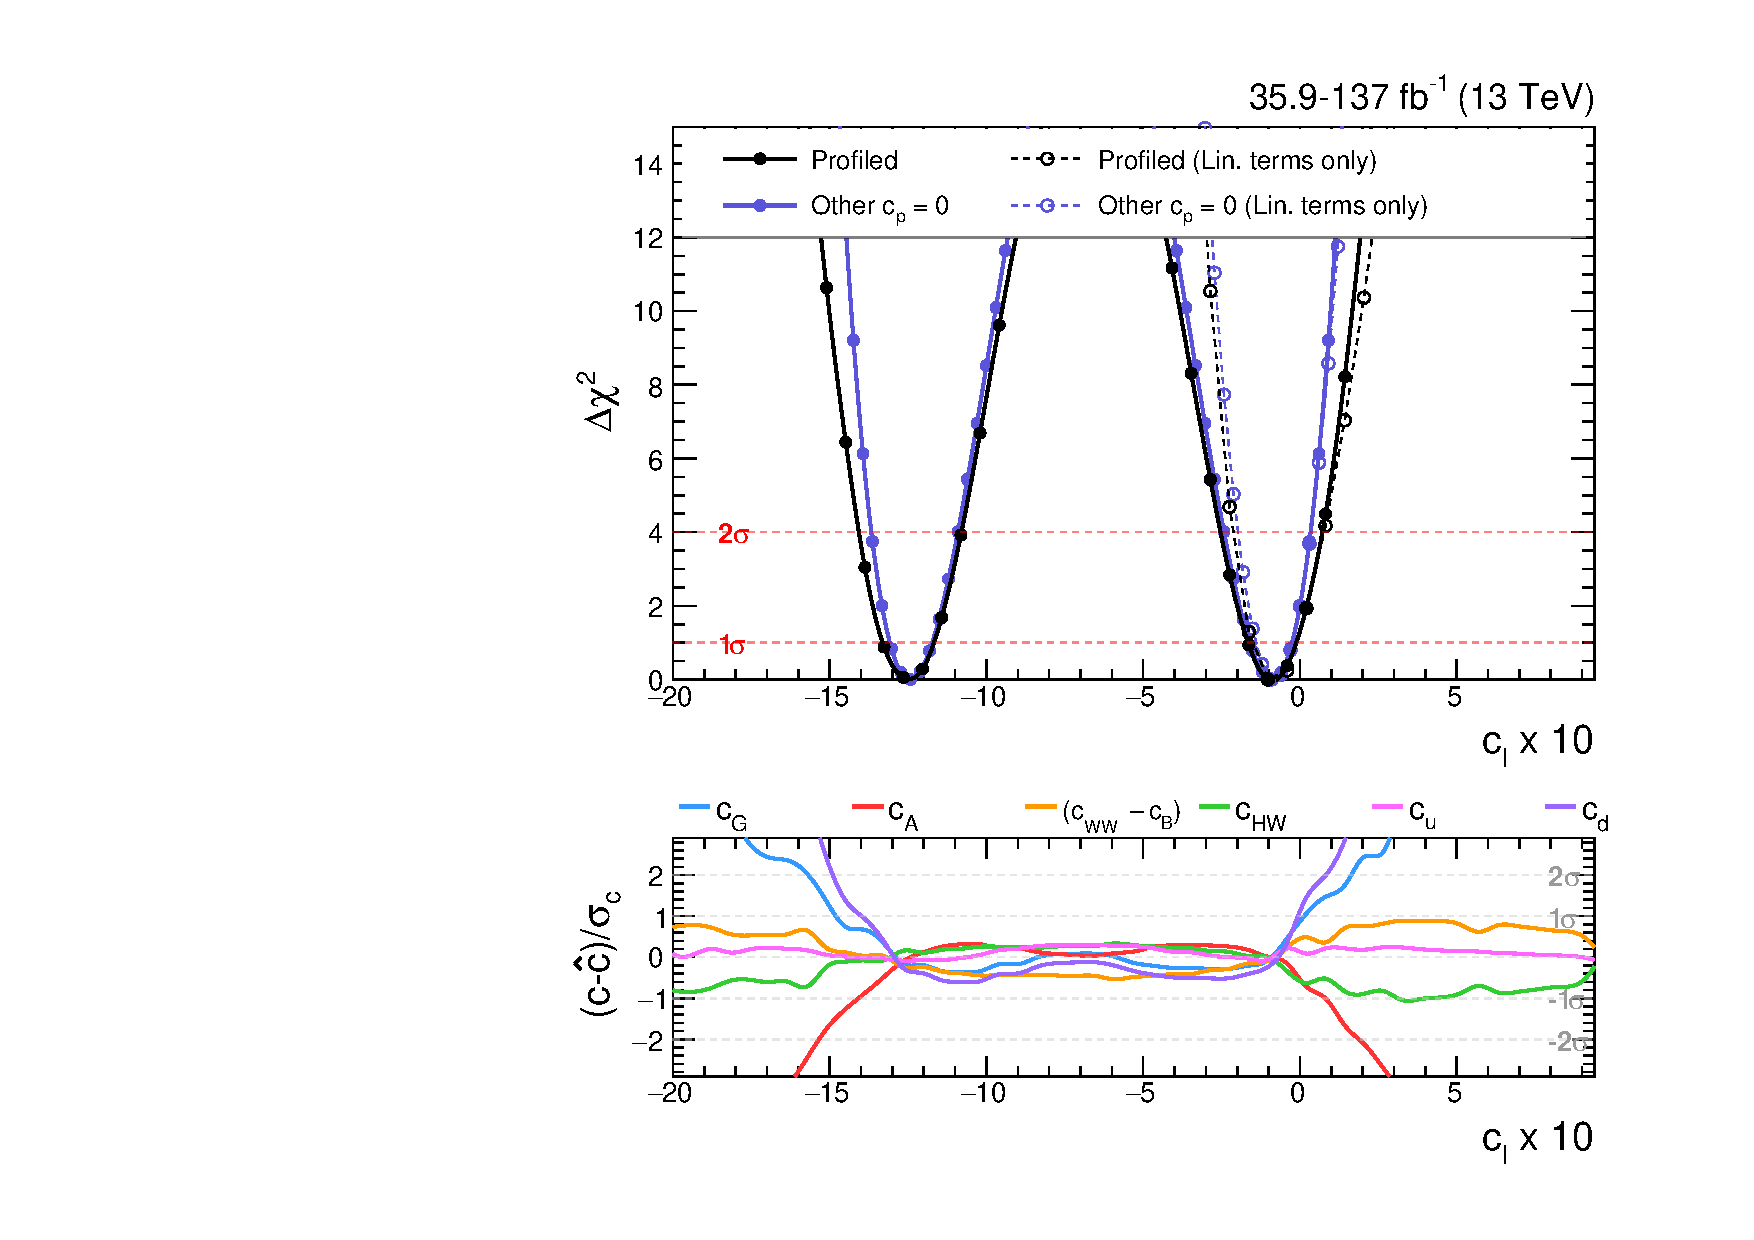
\includegraphics[width=.49\textwidth]{Figures/eft/chi2/observed/cl.pdf}
  \caption[Simplified HEL re-interpretation: $c_u$, $c_d$ and $c_{\ell}$]
  {
    The $\Delta\chi^2(c_p)$ curves for the HEL parameters: $c_u$, $c_d$ and $c_\ell$. The black and purple lines in the top panels correspond to the fits in which the other parameters are profiled and fixed to the SM, respectively. The dashed lines indicate the fits when only linear terms are considered in the parametrisation. The points in each curve show the values of $c_p$ where the minimisation is performed; the lines are extracted by interpolating between these points. The horizontal red lines at $\Delta\chi^2(c_p)=1$ and 4 indicate the $1\sigma$ and $2\sigma$ confidence intervals in $c_p$, respectively. The bottom panels show the pull of the profiled parameters with respect to the parameter of interest. 
  }
  \label{fig:hel_chi2_simplified_1}
\end{figure}
